\section{Derivate}

\dfn{
	Dato un intervallo $I \in \mathbb{R}$, $x_0 \in I$ si dice \textbf{punto 
    interno} a $I$ se \textbf{esiste un intorno sferico:}
	\begin{equation*}
		B_r(x_0) = \{x \in \mathbb{R} \;| \; |x-x_0| < 0\}
	\end{equation*}
	tale che:
	\begin{equation*}
		B_r(x_0) \subseteq I
	\end{equation*}
}
L'insieme dei punti interni si indica con un piccolo \textit{tondino} in alto:
\begin{equation*}
	\mathring{I} := \{x \in I \; | \;\; \text{x è un punto interno a}\;I\} 
\end{equation*}
Questi punti sono diversi rispetto ai punti di accumulazione dei limiti per un 
paio di motivi. Il primo è che devono appartenere innanzitutto all'insieme. Se 
infatti si considera un insieme del tipo $\mathbb{R} \setminus \{0\}$, lo $0$ è 
un punto di accumulazione pur non appartenendo all'insieme. Non è però un punto 
interno. La seconda differenza principale con i punto di accumulazione è che, 
mentre questi ultimi possono essere "al bordo" di un insieme, i punti interni 
no, e devono avere l'intorno sferico completamente interno all'insieme. Cioè 
preso l'intervallo $[2, 4]$, mentre sia $2$ sia $4$ sono punti di 
accumulazione, nessuno dei due è interno all'insieme. In questo caso i punti 
interni a questo insieme sono $]2,4[$.

\subsection{Introduzione informale}
Prima di dare la definizione formale di derivata vorrei spendere qualche riga 
per cercare di spiegare l'idea che si trova dietro a questo potentissimo 
oggetto matematico. Il problema è che spesso ci si perde nelle definizioni 
formali e negli esercizi, senza apprezzare veramente quello che si sta facendo. 
Perché alla fine si spera che ognuno, dopo aver seguito un corso di analisi, 
sappia che la derivata di $x^2$ è $2x$, oppure che la derivata del seno è il 
coseno, però veramente in pochi hanno capito cosa significa e perché è così.\\

\textbf{Derivata come tangente una curva:} Vi siete mai chiesti (probabilmente 
no ma la domanda retorica andava fatta) quale sia la retta tangente a una 
curva? Cioè, se io vi disegno una curva su un foglio e vi traccio un punto 
sopra e vi chiedo di disegnare la tangente a quella curva, probabilmente la 
richiesta non risulta così difficile. Magari la retta non verrà perfetta, però 
il disegno si avvicinerebbe parecchio ad una vera e propria tangente. Se però 
io invece di darvi un disegno di una curva vi do una funzione e un punto, 
trovare la tangente ora è molto più complicato perché dovreste prima disegnare 
la funzione e poi finalmente tracciare la tangente. Però poi nasce il problema 
di come si disegna una funzione in modo abbastanza preciso e quindi la 
situazione diventa piuttosto complicata. 

Facciamo un piccolo salto indietro e chiediamoci prima come si disegna una 
retta. Una retta, nella sua forma più classica, è data dalla seguente formula:
\begin{equation*}
	y = mx + q
\end{equation*}
Abbiamo quindi bisogno di due elementi per definirla: un coefficiente angolare 
$m$ e un termine noto $q$. Sappiamo però, dati due punti, trovare l'unica retta 
che passa per entrambi. Mettiamo di avere $A(x_a, y_a)$ e $B(x_b, y_b)$. 
Innanzitutto troviamo il coefficiente angolare della retta:
\begin{equation*}
	m = \dfrac{y_a - y_b}{x_a - x_b}
\end{equation*}
Fatto questo trovare $q$ non è molto difficile: basta inserire nella retta $m$ 
e uno qualsiasi dei due punti e risolvere l'equazione.

In realtà questo metodo di calcolare la retta presi due punti ci potrebbe 
venire molto comodo per calcolare la tangente ad una curva. Se infatti 
prendiamo due punti su di essa e poi li \textit{avviciniamo abbastanza} tra 
loro possiamo ottenere una buona approssimazione di una tangente (figura 
\ref{fig_approxTangenteCurva}).

\begin{figure}[h]
\centering
\begin{tikzpicture}
\begin{axis}[xmax = 3, xmin = -0.5, ymax = 2, ymin = -0.5,
             axis lines=middle, xlabel=$x$, ylabel=$y$,
             xtick={10},
             ytick={10},
             xlabel style={anchor=north east},
             xticklabel style={anchor=north},
             yticklabel style={anchor=east},
             width=\linewidth,
            ]
\addplot[domain=-1:3, samples=200]{-0.2*x*x + 0.8 * x + 0.4};
\addplot[domain=-1:3, samples=200, dashed]{0.2 * x + 0.65};
\addplot[domain=-1:3, samples=200, dashed]{0.3 * x + 0.6};
\addplot[domain=-1:2.7, samples=200, dashed]{0.5 * x + 0.5};
\addplot[domain=-1:3, samples=200]{0.6 * x + 0.45};
\addplot [only marks, mark options={scale=1}] table {
0.5 0.75
1 1
2 1.2
2.5 1.15
};
\end{axis}
\end{tikzpicture}
  \caption{Approssimazione di una tangente con rette passanti per due punti} 
	\label{fig_approxTangenteCurva}
\end{figure}

Il calcolo difficile non è tanto però il termine noto $q$, ma piuttosto il 
coefficiente angolare $m$. Questo perché dobbiamo prendere punti sempre più 
vicini e non è facile farlo venire preciso. Questo avvicinarci indefinitamente 
ad un punto dovrebbe però far accendere una piccola lampadina in testa: abbiamo 
già uno strumento matematico che ci permette di avvicinarci indefinitamente ad 
un punto: \textbf{il limite}. 

Prendiamo ora una funzione $f(x)$ per il momento generica\footnote{Per 
correttezza questa funzione non può essere generica perché non tutte le 
funzioni sono effettivamente derivabili, però rimaniamo così per il momento. 
In seguito verrà definita rigorosamente.} e decidiamo di voler calcolare la 
tangente nel punto $x_0$. Come abbiamo appena visto ci servono due punti per 
calcolare la tangente: uno che resta fermo (in questo caso $x_0$) e uno che si 
avvicina a quest'ultimo. Per correttezza $x_0$ non è un punto, ma bensì $P(x_0, 
f(x_0))$. Il secondo punto che ci serve deve essere anch'esso sulla funzione e 
quindi imponiamo questa condizione per la sua ordinata: $Q(x, f(x))$. Il 
coefficiente angolare tra i due risulta quindi:
\begin{equation*}
	m = \dfrac{Q_y - P_y}{Q_x - P_x} = \dfrac{f(x) - f(x_0)}{x-x_0}
\end{equation*}
Facendo in modo che il punto $Q$ si avvicini a $P$ indefinitamente:
\begin{equation*}
	\lim_{x \to x_0} \dfrac{f(x) - f(x_0)}{x-x_0}
\end{equation*}
Et voilà, siamo arrivati alla definizione (informale) di derivata. La 
\textit{derivata della funzione $f$ nel punto $x_0$} è proprio il valore di 
quel limite, cioè il \textbf{coefficiente angolare della retta tangente alla 
funzione f nel punto $x_0$}. 

Se si vuole trovare più comodamente la retta tangente una funzione $f(x)$ in un 
punto $x_0$ basta usare la formula:
\begin{equation*}
	y = f'(x_0) (x - x_0) + f(x_0)
\end{equation*}
In generale è inutile comunque impararla perché si può sempre trovare la 
tangente in due passaggi: si calcola la derivata e quindi il coefficiente 
angolare e poi si impone il passaggio per il punto $P(x_0, f(x_0))$ e 
automaticamente si ha la stessa retta.\\

Facciamo un esempio: proviamo a trovare la retta tangente al grafico di $3x^3$ 
nel punto $x = 1$. Iniziamo calcolando la derivata nel punto:
\begin{equation*}
	\lim_{x \to 1} \dfrac{f(x) - f(1)}{x - 1} = \lim_{x \to 1} 
    \dfrac{3x^3 - 3}{x - 1}
\end{equation*}
Raccogliamo il $3$ e usiamo qualche piccolo trucchetto per trovare il limite:
\begin{equation*}
	\lim_{x \to 1} 3 \cdot \dfrac{x^3 - 1}{x - 1} = \lim_{x \to 1} 3 \cdot 
    \dfrac{(x - 1)(x^2 + x + 1)}{x - 1} = \lim_{x \to 1} 3(x^2 + x + 1) = 3 
    \cdot 3 = 9
\end{equation*}
Ne consegue che il coefficiente angolare della retta tangente nel punto $x = 1$ 
è $m = 9$. Imponiamo ora il passaggio per il punto $P(1, f(1)) = P(1, 3)$:
\begin{align*}
	y &= mx + q\\
	3 &= 9 \cdot 1 + q\\
	q &= 3 - 9 = -6
\end{align*}
Ne consegue che la nostra retta ha equazione:
\begin{equation*}
	y = 9x - 6
\end{equation*}


\textbf{Derivata come misura del cambiamento:} Un altro modo di vedere la 
derivata è come \textit{misura del cambiamento}. Successivamente introdurremo 
un teorema che esplicita meglio questo concetto, ma per ora limitiamoci ad 
introdurlo informalmente. Come abbiamo appena visto la derivata è \textit{il 
coefficiente angolare della retta tangente una curva in un punto}. Se 
osserviamo le figure \ref{fig_tangente12} e \ref{fig_tangente3} si può vedere 
come il coefficiente sia proporzionalmente più grande in base a quanto sta 
crescendo (o diminuendo per coefficienti negativi) la funzione. In pratica la 
derivata in questo caso sta rispondendo alla domanda \textbf{quanto sta 
cambiando la funzione in quel punto?} 

\begin{figure}
\centering
\begin{subfigure}{0.49\textwidth}
\centering
	\begin{tikzpicture}
	\begin{axis}[xmax = 5, xmin = -2.5, ymax = 4, ymin = -0.5,
		     axis lines=middle, xlabel=$x$, ylabel=$y$,
		     xtick={10},
		     ytick={10},
		     xlabel style={anchor=north east},
		     xticklabel style={anchor=north},
		     yticklabel style={anchor=east},
		    ]
		\addplot[domain=-3:12, samples=200]{ln(x+5)};
		\addplot[domain=-3:3, samples=200, dashed]{0.1923* x + 1.6101};
		\addplot [only marks, mark options={scale=1}] table {
		0.2 1.648
		};
	\end{axis}
	\end{tikzpicture}
\end{subfigure}
\begin{subfigure}{0.49\textwidth}
\centering
	\begin{tikzpicture}
	\begin{axis}[xmax = 6, xmin = -0.5, ymax = 4, ymin = -0.5,
		     axis lines=middle, xlabel=$x$, ylabel=$y$,
		     xtick={10},
		     ytick={10},
		     xlabel style={anchor=north east},
		     xticklabel style={anchor=north},
		     yticklabel style={anchor=east},
		    ]
		\addplot[domain=-1:6, samples=200]{ln(x)+2};
		\addplot[domain=-1:5, samples=200, dashed]{2/3* x -0.594 + 2};
		\addplot [only marks, mark options={scale=1}] table {
		1.5 2.405
		};
	\end{axis}
	\end{tikzpicture}
\end{subfigure}
\caption{Tangenti una curva, coefficienti angolari rispettivamente (da sinistra 
    a destra) $11^\circ$ e $33^\circ$} 
\label{fig_tangente12}
\end{figure}

\begin{figure}[h]
\centering
\begin{tikzpicture}
\begin{axis}[xmax = 4, xmin = -3, ymax = 10, ymin = -0.5,
             axis lines=middle, xlabel=$x$, ylabel=$y$,
             xtick={10},
             ytick={10},
             xlabel style={anchor=north east},
             xticklabel style={anchor=north},
             yticklabel style={anchor=east},
             width=0.6\linewidth,
            ]
	\addplot[domain=-3:12, samples=200]{x*x};
\addplot[domain=-2:4, samples=200, dashed]{4*x-4};
\addplot[domain=-3:2, samples=200, dashed]{-2*x-1};
\addplot [only marks, mark options={scale=1}] table {
2 4
-1 1
};
\end{axis}
\end{tikzpicture}
\caption{Tangente una curva, coefficiente angolare (da sinistra a destra) 
    $-63^\circ$ e $75^\circ$} 
	\label{fig_tangente3}
\end{figure}

Per quello può essere vista come la misura del cambiamento, perché se derivi 
una funzione puoi scoprire quanto effettivamente quella stia cambiando in 
relazione al suo argomento.

\subsection{Introduzione formale}
\dfn{
	Data una funzione $f: I \to \mathbb{R}$ e un punto $x_0 \in \mathring{I}$, 
    $f$ si dice \textbf{derivabile in $x_0$} se:
	\begin{equation*}
		\exists \lim _{x \to x_0} \dfrac{f(x) - f(x_0)}{x - x_0} \in \mathbb{R}
	\end{equation*}
	Ci sono due principali notazioni per indicare la derivata della funzione 
    $f$ nel punto $x_0$:
	\begin{equation*}
		f'(x_0) \quad \text{oppure} \quad \dv{f}{x} \left(x_0\right)
	\end{equation*}
	In generale i matematici preferiscono la prima mentre i fisici la seconda.
}
Essendo che $c$ si sta avvicinando a $x_0$, è possibile riscrivere la derivata 
in maniera differente: In pratica $x$ lo scriviamo in funzione di $x_0$ e ci 
aggiungiamo una piccola variabile che diventa sempre più piccola. Il risultato 
è lo stesso ma a per certe dimostrazioni conviene scriverlo così:
\begin{equation*}
	\lim_{h \to 0} \dfrac{f(x + h) - f(x)}{h}
\end{equation*}

Infatti $x_0 = x + h$ e il denominatore si semplifica in quanto $x - x_0 = x - 
x - h = -h$. Cambiando segno anche al numerato il risultato è lo stesso.

\dfn{
	Derivata destra e sinistra: $f: I \to \mathbb{R}$, $x_0 \in \mathring{I}$. 

	\begin{itemize}
		\item $f$ si dice \textbf{derivabile a sinistra in $x_0$}, e si indica 
            $f'_-(x_0)$, se:
			\begin{equation*}
				\exists \lim _{x \to x_0^-} \dfrac{f(x) - f(x_0)}{x - x_0} \in 
                \mathbb{R} 
			\end{equation*}

		\item $f$ si dice \textbf{derivabile a destra in $x_0$}, e si indica 
            $f'_+(x_0)$, se:
			\begin{equation*}
				\exists \lim _{x \to x_0^+} \dfrac{f(x) - f(x_0)}{x - x_0} \in 
                \mathbb{R} 
			\end{equation*}
	\end{itemize}
}

L'idea è la stessa dei limiti:
\begin{equation*}
	f \; \text{è derivabile in } x_0 \iff
	\begin{cases*}
		f \; \text{è derivabile sia a destra che a sinistra di } x_0\\
		f'_+(x_0) = f'_-(x_0) = f(x_0)
	\end{cases*}
\end{equation*}

\dfn{
	$f$ si dice \textbf{derivabile su} $I$ se $f$ è derivabile $\forall x \in 
    I$
}
In questo ultimo caso, ad $f$ si può associare una nuova funzione: la sua 
derivata. In pratica la nuova funzione assume i valori della derivata di $f$ 
per ogni punto in cui è definita. Si indica generalmente con la notazione 
classica $f'(x)$.\\

\textbf{Alcuni esempi:} Di seguito riporto qualche esempio molto semplice di 
calcolo della derivata tramite la sua definizione. In realtà raramente si usa 
questo approccio nei calcoli effettivi, ma piuttosto si ricavano prima le 
derivate delle funzioni elementari e applicando qualche regola si riesce a 
derivare qualsiasi funzione senza calcolare limiti. È bello però far vedere 
comunque la definizione e la sua potenza in quanto tutto quello che verrà dopo 
sarà comunque frutto di questo.

Proviamo a derivare $f(x) = x$:
\begin{equation*}
	\lim_{h \to 0} \dfrac{f(x_0 + h) - f(x_0)}{h} = \lim_{h \to 0} \dfrac{x_0 
    + h -x_0}{h} = \lim_{h \to 0} 1 = 1
\end{equation*}

Quindi $f'(x) = 1$. È facile verificare che questo è vero perché la funzione 
$x$ è semplicemente una retta, che ha lo stesso coefficiente angolare $\forall 
x \in \mathbb{R}$. Inoltre alla domanda "\textit{quanto sta cambiando questa 
funzione?}" è facile vedere che la funzione cambia sempre nello stesso modo, 
quindi il valore della sua derivata è costante.

La funzione costante $g(x) = k$ invece che derivata ci aspettiamo che abbia? 
In teoria, essendo costante, la funzione non cambia mai. Quindi possiamo 
aspettarci che la sua derivata sia nulla. Verifichiamolo:
\begin{equation*}
	\lim_{h \to 0} \dfrac{f(x_0 + h) - f(x_0)}{h} = \lim_{h \to 0} 
    \dfrac{5 - 5}{h} = 0
\end{equation*}
In questo caso il limite non è una forma indeterminata perché il numeratore è 
\textbf{esattamente} $0$, mentre il denominatore si avvicinerà sempre di più a 
quel valore, ma non lo raggiungerà mai (come da definizione di limite).

Proviamo a derivare una funzione leggermente più complessa: $h(x) = x^2$ :
\begin{align*}
	&\lim_{h \to 0} \dfrac{f(x_0 + h) - f(x_0)}{h} = \lim_{h \to 0} 
    \dfrac{(x+h)^2 - x^2}{h} =  \lim_{h \to 0} \dfrac{x^2 +2 x h + h^2 - 
    x^2}{h} =\\
	&\lim_{h \to 0} \dfrac{2xh + h^2}{h} = \lim_{h \to 0} 2x + h =  2x
\end{align*}

La derivata in questo caso risulta essere $2x$. Ed effettivamente ha senso 
visto che il grafico di $x^2$ cambia sempre di più all'aumentare di $x$. Se 
infatti si guarda la classica forma di una parabola si può facilmente notare 
che più aumenta $x$, più il grafico \textit{acquista pendenza}.



\subsection{Regole di derivazione} \label{sec_regoleDerivazione}
È oggettivamente infattibile derivare ogni singola funzione con la definizione 
di derivata. Di conseguenza tramite questa ultima si ricavano delle piccole 
regoline che permettono poi di semplificare enormemente il calcolo:
\imp{
\begin{enumerate}
	\item Costante per una funzione:
		\begin{equation*}
			(a \cdot f)' = a \cdot f'(x)
		\end{equation*}
	\item Somma e sottrazione di funzioni:
		\begin{equation*}
			(f \pm g)' = f' \pm g'
		\end{equation*}

	\item Prodotto di funzioni:
		\begin{equation*}
			(f \cdot g)' = f' \cdot g + f \cdot g'
		\end{equation*}

	\item Quoziente di funzioni:
		\begin{equation*}
			\left( \dfrac{f}{g} \right)' = \dfrac{f' \cdot g - f \cdot g'}{g^2}
		\end{equation*}

	\item Composizione di funzioni
		\begin{equation*}
			(f \circ g)' = (f' \circ g) \cdot g'
		\end{equation*}
		Il simbolo $\circ$ indica la composizione di funzioni, cioè $f \circ g 
        = f(g(x))$.
\end{enumerate}
}

\subsection{Algebra delle derivate} 
Questa sottosezione sembrerà un duplicato delle regole di derivazione (Sezione: 
\ref{sec_regoleDerivazione}). In parte lo è, ma in realtà vuole rendere più 
formali quelle regole che hanno qualche piccola premessa volutamente mancante 
ma che in teoria dovrebbe averle rese più chiari e semplici da leggere.\\

Date due funzioni $f, g: I \to \mathbb{R}$, e un punto $x_0 \in I$, se $f$ e 
$f$ sono derivabili in $x_0$ allora:
\begin{enumerate}
	\item $f \pm g$ è derivabile in $x_0$ e: 
		\begin{equation*}
			(f \pm g)' (x_0) = f'(x_0) \pm g'(x_0)
		\end{equation*}

	\item $f \cdot g$ è derivabile in $x_0$ e: 
		\begin{equation*}
			(f \cdot g)' (x_0) = f'(x_0) \cdot g(x_0) + f(x_0) \cdot g'(x_0)
		\end{equation*}

	\item $\dfrac{f}{g}$ è derivabile in $x_0$ se $g(x_0) \neq 0$ e: 
		\begin{equation*}
			\left( \dfrac{f}{g} \right)' = \dfrac{f' \cdot g - f \cdot g'}{g^2}
		\end{equation*}
\end{enumerate}
\thm{
	Dati due intervalli $I, J \subseteq \mathbb{R}$, due funzioni $f:I \to 
    \mathbb{R}$ e $g: J \to I$ e un punto $x_0 \in J$. Se $g$ è derivabile 
    in $x_0$ e $f$ è derivabile in $g(x_0)$ allora $f \circ g$ è derivabile 
    in $x_0$ e vale:

	\begin{equation*}
		(f \circ g)' (x_0) = f'(g(x_0)) \cdot g'(x_0)
	\end{equation*}
}

\subsection{Derivate funzioni elementari} 
\imp{
\begin{multicols}{2}
\begin{itemize}
	\item $(x^n)' = nx^{n-1}$ 

	\item $(e^x)' = e^x$
	\item $(a^x)' = a^x \cdot \ln(a)$ con $a > 0$

	\item $(\ln(x))' = \dfrac{1}{x}$
	\item $(\log_a (x))' = \dfrac{1}{x \cdot ln(a)}$

	\item $(\sin(x))' = \cos(x)$
	\item $(\cos(x))' = -\sin(x)$
	\item $(\tan(x))' = \dfrac{1}{\cos^2(x)} = 1 + \tan^2(x)$

	\item $(\arcsin(x))' = \dfrac{1}{\sqrt{1 - x^2}}$
	\item $(\arccos(x))' = -\dfrac{1}{\sqrt{1 - x^2}}$
	\item $(\arctan(x))' = \dfrac{1}{1 + x^2}$
\end{itemize}
\end{multicols}
}

Di seguito sono presenti le dimostrazioni di alcune di queste derivate:
\pf{
	Dobbiamo dimostrare:
	\begin{equation*}
		(x^n)' = n \cdot x^{n - 1} \qquad \forall x \in \mathbb{N}
	\end{equation*}
	Prendiamo una funzione $f(x) = x^n$ con $n \in \mathbb{N}$ e $n > 2$. Ci 
    riduciamo a dimostrare quindi:
	\begin{equation*}
		f'(x) = n \cdot x^{n-1}
	\end{equation*}
	Ora dalla definizione di derivata:
	\begin{equation*}
		f'(x) = \lim_{h \to 0} \dfrac{f(x + h) - f(x)}{h} = \lim_{h \to 0} 
        \dfrac{(x + h)^n - x^n}{h}
	\end{equation*}
	Dal binomio di newton (Sezione \ref{sec_binomioNewton}):
	\begin{equation*}
		(x + h)^n = \sum \limits_{j = 0}^n \binom{n}{j} \cdot x^{n-j} \cdot h^j 
        = x^n + \binom{n}{1} \cdot x^{n-1} \cdot h + \sum_{j = 2}^{n} 
        \binom{n}{j} x^{n -j} \cdot h^j
	\end{equation*}
	Essendo $\binom{n}{1} = n$, possiamo sostituire nel limite:
	\begin{align*}
		&\lim_{h \to 0} \dfrac{x^n + n \cdot x^{n-1} \cdot h + \sum_{j = 2}^{n} 
        \binom{n}{j} x^{n -j} \cdot h^j - x^n}{h} =\\[10pt]
		=& \lim_{h \to 0} \left( n \cdot x^{n-1} + \sum_{j = 2}^n \binom{n}{j} 
        x^{n-j} \cdot h^{j-1} \right)
	\end{align*}
	L'esponente di $h$, essendo che la sommatoria parte da $j = 2$, sarà sempre 
    maggiore o uguale a uno ($j-1 \geq 1$). Di conseguenza essendo $h \to 0$ 
    per il limite, tutta la sommatoria va a $0$:
	\begin{equation*}
		n \cdot x^{n-1}
	\end{equation*}

	\hfill Qed.
	
}
In questo caso abbiamo trovato la derivata di $x^n$ ma solo per $n \in 
\mathbb{N}$. In realtà possiamo provare che è la stessa identica cosa però per 
$n \in \mathbb{R}$:
\pf{
	Dobbiamo dimostrare:
	\begin{equation*}
		(x^n)' = n \cdot x^{n - 1} \qquad \forall x \in \mathbb{R}
	\end{equation*}
	Prendiamo una funzione $f(x) = x^n$ con $n \in \mathbb{R}$ e $n > 0$. Ora 
    usando sia l'esponenziale che il logaritmo in quanto sua inversa possiamo 
    riscrivere la funzione come:
	\begin{equation*}
		f(x) = x^n = e^{\ln(x^n)} = e^{n \cdot \ln{x}}
	\end{equation*}
	Questa ultima è derivabile per $x > 0$. Calcoliamo quindi la derivata:
	\begin{equation*}
		f'(x) = \left( e^{n \cdot \ln{x}} \right)' = e^{n \cdot \ln{x}} \cdot 
        (n \cdot \ln{x})' = x^n \cdot n \cdot \dfrac{1}{x} = n \cdot x^{n-1}
	\end{equation*}
	\hfill Qed.
}

\pf{
	Dobbiamo provare che:
	\begin{equation*}
		(\sin (x))' = \cos(x)
	\end{equation*}
	Chiamiamo $f(x) = \sin (x)$ e applichiamo la definizione:
	\begin{equation*}
		f'(x) = \lim_{h \to 0} \dfrac{f(x + h) - f(x)}{h} = \lim_{h \to 0} 
        \dfrac{\sin(x + h) - \sin(x)}{h}
	\end{equation*}
	Usando le formule di addizione (Sezione \ref{sec_formuleAddSott}):
	\begin{align*}
		&\lim_{h \to 0} \dfrac{\sin(x)\cos(h) + \cos(x)\sin(h) - \sin(x)}{h} = 
        \lim_{h \to 0} \dfrac{\sin(x) \cdot (\cos(h) -1) + \cos(x)\sin(h)}{h} 
        =\\[10pt]
		= &\lim_{h \to 0} \sin(x) \cdot \dfrac{\cos(h) - 1}{h} + \cos(x) \cdot 
        \dfrac{\sin(h)}{h}
	\end{align*}
	Usando qualche limite notevole visto in precedenza (Sezione 
    \ref{sec_limitiNotevoli}):
	\begin{equation*}
		\lim_{h \to 0} \sin(x) \cdot 0 + \cos(x) \cdot 1 = \cos(x)
	\end{equation*}
	\hfill Qed.
}

\pf{
	Dobbiamo provare che:
	\begin{equation*}
		(\cos (x))' = -\sin(x)
	\end{equation*}
	Chiamiamo $f(x) = \cos (x)$ e applichiamo la definizione:
	\begin{equation*}
		f'(x) = \lim_{h \to 0} \dfrac{f(x + h) - f(x)}{h} = \lim_{h \to 0} 
        \dfrac{\cos(x + h) - \cos(x)}{h}
	\end{equation*}
	Usando le formule di addizione (Sezione \ref{sec_formuleAddSott}):
	\begin{align*}
		&\lim_{h \to 0} \dfrac{\cos(x)\cos(h) - \sin(x)\sin(h) - \cos(x)}{h} = 
        \lim_{h \to 0} \dfrac{\cos(x) \cdot (\cos(h) -1) - \sin(x)\sin(h)}{h} 
        =\\[10pt]
		= &\lim_{h \to 0} \cos(x) \cdot \dfrac{\cos(h) - 1}{h} - \cos(x) \cdot 
        \dfrac{\sin(h)}{h}
	\end{align*}
	Usando qualche limite notevole visto in precedenza (Sezione 
    \ref{sec_limitiNotevoli}):
	\begin{equation*}
		\lim_{h \to 0} \cos(x) \cdot 0 - \sin(x) \cdot 1 = -\sin(x)
	\end{equation*}
	\hfill Qed.

}
\pf{
	Dobbiamo provare che:
	\begin{equation*}
		(\tan(x))' = \dfrac{1}{\cos^2(x)} = 1 + \tan^2(x)
	\end{equation*}
	In questo caso essendo:
	\begin{equation*}
		\tan(x) = \dfrac{\sin(x)}{\cos(x)}
	\end{equation*}
	Ci basta calcolare la derivata di un quoziente:
	\begin{equation*}
		(\tan(x))' = \left( \dfrac{\sin(x)}{\cos(x)} \right)' = 
        \dfrac{\cos(x)\cos(x) - \sin(x) \cdot -\sin(x)}{\cos^2(x)} = 
        \dfrac{\cos^2(x) + \sin^2(x)}{\cos^2(x)}
	\end{equation*}
	Che in base a come si vuole semplificare porta a due possibili risultati:
	\begin{enumerate}
		\item 
			\begin{equation*}
				\dfrac{\cos^2(x) + \sin^2(x)}{\cos^2(x)} = \dfrac{1}{\cos^2(x)}
			\end{equation*}

		\item 
			\begin{equation*}
				\dfrac{\cos^2(x) + \sin^2(x)}{\cos^2(x)} = 
                \dfrac{\cos^2(x)}{\cos^2(x)} + \dfrac{\sin^2(x)}{\cos^2(x)} = 
                1 + \tan^2(x)
			\end{equation*}
	\end{enumerate}
	
}

\subsection{Derivare un valore assoluto}
Proviamo a derivare il valore assoluto di $x$:
\begin{equation*}
    f(x) = |x| =
    \begin{cases*}
        x \quad \;\;\, \text{se} \quad x \geq 0\\
        -x \quad \text{se} \quad x < 0
    \end{cases*}
\end{equation*}
È abbastanza facile vedere che è derivabile sicuramente per tutto l'intervallo 
$\mathbb{R} \setminus \{0\}$ perché se prese singolarmente, sia $x$ che $-x$ 
sono derivabili. Il problema è che non sappiamo se è derivabile in $x = 0$. 
Usiamo la definizione approcciando questa derivata prima da sinistra e poi da 
destra:
\begin{equation*}
	f_-' (0) \lim_{x \to 0^-} \dfrac{f(x) - f(0)}{x -0} = \lim_{x \to 0^-} 
    \dfrac{|x|}{x}
\end{equation*}
Essendo che ci stiamo avvicinando a $0$ da sinistra ($x \to 0^-$), il valore 
assoluto è semplicemente $-x$:
\begin{equation*}
	\lim_{x \to 0^-} \dfrac {-x}{x} = -1
\end{equation*} 
Usando lo stesso procedimento per la derivata destra:
\begin{equation*}
	f_+' (0) \lim_{x \to 0^+} \dfrac{f(x) - f(0)}{x -0} = \lim_{x \to 0^+} 
    \dfrac{|x|}{x} = \lim_{x \to 0^+} \dfrac {x}{x} = 1
\end{equation*}
Concludiamo quindi che $|x|$ \textbf{non è derivabile} in $x = 0$ perché il 
valore della sua derivata destra non coincide con il valore della derivata 
sinistra:
\begin{equation*}
	f_-' (0) = -1 \; \neq \; 1 = f_+'(0)
\end{equation*}

In generale però \textbf{il valore assoluto in una funzione non rende per forza 
questa non derivabile}. Un classico esempio è:
\begin{equation*}
	g(x) = x|x| = 
	\begin{cases*}
		x^2 \quad \;\;\, \text{se} \quad x \geq 0\\
		-x^2 \quad \text{se} \quad x < 0
	\end{cases*}
\end{equation*}
Se si considera sempre l'intervallo $\mathbb{R} \setminus \{0\}$ è facile 
notare che presi distintamente, i due tratti della funzione sono derivabili. 
Il problema resta sempre però il punto $x = 0$. Approcciamolo da sinistra:
\begin{equation*}
	\lim_{x \to 0^-} \dfrac{f(x) - f(0)}{x - 0} = \lim_{x \to 0^-} 
    \dfrac{-x^2}{x} = \lim_{x \to 0^-} -x = 0
\end{equation*}
Approcciamolo ora da destra:
\begin{equation*}
	\lim_{x \to 0^+} \dfrac{f(x) - f(0)}{x - 0} = \lim_{x \to 0^+} 
    \dfrac{x^2}{x} = \lim_{x \to 0^+} x = 0
\end{equation*}
Ne consegue che \textbf{la funzione è derivabile} proprio perché la sua 
derivata destra e sinistra coincidono.

\subsection{Derivate di ordine superiore}
L'idea dietro le derivate di ordine superiore è il fatto che la funzione 
derivata di una qualsiasi funzione resta comunque una funzione. Cioè se scrivo:
\begin{equation*}
	3x^2 + 4
\end{equation*}
Non esiste modo di distinguere se questa è una derivata o una funzione proprio 
perché non c'è differenza tra queste due. Se fosse una derivata la funzione 
potrebbe essere tipo questa\footnote{In realtà ci possono essere infinite 
funzioni che hanno la seguente come derivata, ma è un discorso che va 
affrontato poi con gli integrali}:
\begin{equation*}
	f(x) = x^3 + 4x + 1
\end{equation*}
Ma potrebbe benissimo essere una funzione a parte e si scriverebbe come:
\begin{equation*}
	g(x) = 3x^2 + 4
\end{equation*}
Essendo quindi che la funzione derivata (si capisce anche dal nome) rimane 
comunque una normalissima funzione possiamo applicare nuovamente il concetto di 
derivata alla derivata stessa. Prendiamo per esempio una funzione e deriviamola 
una volta:
\begin{align*}
	j(x) &= 2x^5 - 3x^3 + 5x\\
	j'(x) &= 10x^4 - 9x^2 +5
\end{align*}
Ora possiamo applicare nuovamente il concetto di derivata alla derivata stessa 
(cioè $j'$):
\begin{equation*}
	j''(x) = 40x^3 - 18x
\end{equation*}
In questo caso abbiamo usato due volte il simbolo di derivata $'$ per indicare 
proprio il fatto che è una funzione derivata 2 volte. Ovviamente questa cosa si 
può iterare finché la funzione resta derivabile. Formalizziamo meglio il 
concetto:
\dfn{
	Data una funzione $f: I \to \mathbb{R}$ derivabile su $I$, esiste la 
    derivata $f': I \to \mathbb[R]$. Se $f'$ è derivabile in $x_0 \in I$ 
    allora:
	\begin{equation*}
		f''(x_0) := \lim_{h \to 0} \dfrac{f'(x_o + h) - f'(x_0)}{h} \in R
	\end{equation*}
}
In questo caso si dice che la funzione $f$ \textbf{è derivabile due volte in} 
$\mathbf{x_0}$.

Ne consegue che se volgiamo definire la derivata terza di una funzione in un 
punto $x_0$, basta che esista la derivata seconda della funzione in quel punto 
e che questa ultima si derivabile:
\begin{equation*}
		f'''(x_0) := \lim_{h \to 0} \dfrac{f''(x_o + h) - f''(x_0)}{h} \in R
\end{equation*}

\textbf{Notazioni}:
\begin{gather*}
	f', f'', f''', f^{IV}, f^{V} \cdots\\
	f^{(1)}, f^{(2)}, f^{(3)}, f^{(4)}, f^{(5)}, \cdots
\end{gather*}
\textbf{Nota}: La derivata $f'$ viene spesso chiamata \textit{derivata prima}.

\dfn{
	\textbf{Classe} $\mathbf{C^k}$ dove $k \in \mathbb{N}$. 
	\begin{equation*}
		f \in C^k (I) \iff
		\begin{cases*}
			f \; \text{è derivabile k-volte su } I\\
			f^{(k)} \text{è continua su I}
		\end{cases*}
	\end{equation*}
}
Ci basta imporre solo che $f^{(k)}$ sia continua da un teorema enunciato più 
avanti (Sezione \ref{theorem_DerivataContinua}) che in pratica afferma che se 
una funzione è derivabile (e tutte quelle prima di $f^{(k)}$ lo sono) allora la 
funzione è forza continua.\\

Le classi risultano quindi:
\begin{align*}
	C^0 (I) &= \{f: I \to \mathbb{R}\; |\; f \; \text{continua su I}\}\\
	C^1 (I) &= \{f: I \to \mathbb{R}\; |\; f \; \text{è derivabile e } f':I \to 
    \mathbb{R} \text{ è continua}\}\\
	C^2 (I) &= \{f: I \to \mathbb{R}\; |\; f \; \text{è derivabile due volte 
    e } f'':I \to \mathbb{R} \text{ è continua}\}\\
	\vdots\\
	C^\infty (I) &:= \bigcap_{k} C^k (I)
\end{align*}
L'ultima classe comprende tutte le funzioni derivabili un numero arbitrario di 
volte.\\

Un esempio di funzione derivabile $k$ volte:
\begin{equation*}
	h(x) = x^k |x|  
\end{equation*}
Infatti $h \in C^k (\mathbb{R})$ ma $h \not \in C^{k+1} (\mathbb{R})$.

\subsection{Teoremi}

\thm{ \label{theorem_DerivataContinua}
	Data una funzione $f: I \to \mathbb{R}$ dove $I \subseteq \mathbb{R}$ e un 
    punto $x_0 \in \mathbb{R}$ si ha che:
	\begin{equation*}
		f \; \text{derivabile in } x_0 \implies f \; \text{è continua in } x_0
	\end{equation*}
}
\pf{
	Assumendo che $x_0$ faccia parte dei punti di accumulazione di $I$ ($x_0 
    \in \mathcal{D}(I)$), dobbiamo dimostrare che:
	\begin{equation*}
		\lim_{x \to x_0} f(x) = f(x_0)
	\end{equation*}
	o equivalentemente:
	\begin{equation*}
		\lim_{x \to x_0} [f(x) - f(x_0)] = 0
	\end{equation*}
	Moltiplicando e dividendo per lo stesso fattore ($x - x_0$):
	\begin{equation*}
		\lim_{x \to x_0} \dfrac{f(x) - f(x_0)}{x-x_0} \cdot (x - x_0) = 0
	\end{equation*}
	Il primo termine è semplicemente la derivata di $f$ nel punto $x_0$ mentre 
    il secondo termine tende a zero per $x \to x_0$:
	\begin{equation*}
		f'(x_0) \cdot 0 = 0
	\end{equation*}
	\hfill Qed.
}
È importante notare qui la direzione dell'implicazione: mentre se una funzione 
è derivabile allora è continua, NON è affatto detto che una funzione continua 
automaticamente sia derivabile. L'esempio classico è il valore assoluto di $x$, 
che è continuo su tutto $\mathbb{R}$ ma non è derivabile in $x = 0$. Si può 
vedere la cosa come se le funzioni derivabili fossero un sottoinsieme delle 
funzioni continue.


\subsubsection{Teorema di Fermat} \label{theorem_fermat}
\dfn{
	$f: A \to \mathbb{R}$ 
	\begin{enumerate}
		\item $x_0 \in A$ si dice punti di \textbf{massimo relativo} (o locale) 
            se:
			\begin{equation*}
				\exists r >0: \;\; f(x) \leq f(x_0) \;\; \forall x \in A \cap 
                I_r(x_0)
			\end{equation*}

		\item $x_0 \in A$ si dice punti di \textbf{minimo relativo} (o locale) 
            se:
			\begin{equation*}
				\exists r >0: \;\; f(x) \geq f(x_0) \;\; \forall x \in A \cap 
                I_r(x_0)
			\end{equation*}
	\end{enumerate}
}
In pratica basta che esista un intorno di quel punto in cui tutti i valori 
della funzione sono più piccoli del valore della funzione nel punto stesso per 
fare in modo che quel punto sia un massimo relativo. La stessa cosa vale con il 
minimo. La differenza con i punti di massimo e di minimo assoluti è che questi 
ultimi devono essere maggiori o minori di tutti gli altri valori della 
funzione, non soltanto in un intorno scelto a piacere. Nonostante siano già 
scritti in precedenza riporto nuovamente la definizione:

Data una funzione $f:A \to \mathbb{R}$:
\begin{enumerate}
    \item $x_0 \in A$ si dice punto di \textbf{massimo assoluto} di $f$ se:
    \begin{equation*}
        f(x) \leq f(x_0) \quad \forall x \in A
    \end{equation*}
    
    \item $x_0 \in A$ si dice punto di \textbf{minimo assoluto} di $f$ se:
    \begin{equation*}
        f(x) \geq f(x_0) \quad \forall x \in A
    \end{equation*}
\end{enumerate}

Ovviamente: \\
\begin{align*}
	x_0 \; \text{punto di massimo assoluto} &\implies x_0 \; \text{punto di 
    massimo relativo}\\
	x_0 \; \text{punto di minimo assoluto} &\implies x_0 \; \text{punto di 
    minimo relativo}
\end{align*}

Il seguente teorema enuncia che la derivata nei minimi e nei massimi relativi 
si annulla. Questo teorema torna molto utile nello studio di funzione per 
individuare potenziali massimi o minimi.
\thm {
Data una funzione $f: [a,b] \to \mathbb{R}$, un punto di massimo o di 
minimo $x_0 \in ]a,b[$, se inoltre $f$ è derivabile in $x_0$, allora:
\begin{equation*}
    f'(x_0) = 0
\end{equation*}
}
È essenziale che il punto $x_0$ si all'interno dell'intervallo. Se infatti non 
lo fosse (come da Figura: \ref{fig_fermat1}) la derivata non si annullerebbe 
nonostante gli estremi siano un punto di massimo e di minimo. 

\begin{figure}[h]
\centering
\begin{tikzpicture}
\begin{axis}[xmax = 3, xmin = -0.5, ymax = 8, ymin = -0.5,
             axis lines=middle, xlabel=$x$, ylabel=$y$,
             xtick={10},
             ytick={10},
             xlabel style={anchor=north east},
             xticklabel style={anchor=north},
             yticklabel style={anchor=east},
             width=0.5\linewidth,
            ]
\addplot[domain=0.5:2.2, samples=200]{3 * x};
\addplot [only marks, mark options={scale=1}] table {
0.5 1.5
2.2 6.6
};
\end{axis}
\end{tikzpicture}
  \caption{Caso del teorema di Fermat in cui il punto di massimo o di minimo 
    non è interno all'intervallo e quindi la derivata non si annulla} 
	\label{fig_fermat1}
\end{figure}



Inoltre l'annullarsi della derivata prima in un punto $x_0$ è condizione 
\textbf{necessaria} affinché $x_0$ sia un punto di massimo o di minimo 
relativo, ma \textbf{non è sufficiente} in generale. Se prendiamo infatti la 
funzione $f(x) = x^3$ e la deriviamo viene $f'(x) = 3x^2$ ed è facile vedere 
che la derivata di annulla in $x = 0$. Se guardiamo il grafico di $f(x)$ 
(Figura: \ref{fig_graficoXTree}) però in $x= 0$ non è presente né un massimo 
né un minimo.

\begin{figure}[h]
\centering
\begin{tikzpicture}
\begin{axis}[xmax = 3, xmin = -3, ymax = 9, ymin = -9,
             axis lines=middle, xlabel=$x$, ylabel=$y$,
             xtick={10},
             ytick={10},
             xlabel style={anchor=north east},
             xticklabel style={anchor=north},
             yticklabel style={anchor=east},
             width=0.5\linewidth,
            ]
\addplot[domain=-3:3, samples=200]{x*x*x};
\addplot [only marks, mark options={scale=1}] table {
0 0 
};
\end{axis}
\end{tikzpicture}
	\caption{Grafico della funzione $f(x) = x^3$}
	\label{fig_graficoXTree}
\end{figure}
	

\pf{
	Dimostriamo il teorema solo per il caso dei punti di massimo. Prendiamo una 
    funzione $f:[a, b] \to \mathbb{R}$ che ha un punto di massimo relativo in 
    $x_0 \in ]a, b[$. Assumiamo inoltre che $f$ sia derivabile in $x_0$. 

	Essendo $x_0$ un punto di massimo relativo:
	\begin{equation*}
		\exists r >0: \;\; f(x) \leq f(x_0) \;\; \forall x \in A \cap I_r(x_0)
	\end{equation*}
	L'intorno $I_r(x_0)$ si può scrivere anche come:
	\begin{equation*}
		x_0 - r < x < x_0 + r
	\end{equation*}
	Dividiamo quindi questo intervallo in due casi distinti:
	\begin{enumerate}
		\item Il primo caso considera l'intervallo ristretto a: 
			\begin{equation*}
				x_0 - r < x < x_0
			\end{equation*}
			La derivata sinistra di $f$ nel punto $x_0$ esiste per ipotesi ed è 
            per definizione:
			\begin{equation*}
				f_-'(x_0) = \lim_{x \to x_0^-}  \dfrac{f(x) - f(x_0)}{x-x_0}
			\end{equation*}
			Per ipotesi abbiamo che $f(x) - f(x_0) \leq 0$ e per il fatto che 
            ci stiamo avvicinando a $x_0$ da sinistra $x - x_0 < 0$. Ne 
            consegue che:
			\begin{equation*}
				\dfrac{f(x) - f(x_0)}{x-x_0} \geq 0
			\end{equation*}
			E quindi per il teorema di permanenza del segno (Sezione 
            \ref{theorem_permanenzaSegno}):
		
			\begin{equation*}
				f_-'(x_0) = \lim_{x \to x_0^-}  \dfrac{f(x) - f(x_0)}{x-x_0} 
                \geq 0
			\end{equation*}
			E quindi:
			\begin{equation*}
				f_-'(x_0) \geq 0
			\end{equation*}

		\item Il secondo caso considera l'altro pezzo di intervallo:
			\begin{equation*}
				x_0< x < x_0 + r
			\end{equation*}
			La derivata destra di $f$ nel punto $x_0$ esiste per ipotesi ed è 
            per definizione:
			\begin{equation*}
				f_+'(x_0) = \lim_{x \to x_0^+}  \dfrac{f(x) - f(x_0)}{x-x_0}
			\end{equation*}
			Per ipotesi abbiamo che $f(x) - f(x_0) \leq 0$ e per il fatto che 
            ci stiamo avvicinando a $x_0$ da destra $x - x_0 > 0$. Ne consegue 
            che:
			\begin{equation*}
				\dfrac{f(x) - f(x_0)}{x-x_0} \leq 0
			\end{equation*}
			E quindi per il teorema di permanenza del segno (Sezione 
            \ref{theorem_permanenzaSegno}):
			\begin{equation*}
				f_+'(x_0) = \lim_{x \to x_0^+}  \dfrac{f(x) - f(x_0)}{x-x_0} 
                \leq 0
			\end{equation*}
			E quindi:
			\begin{equation*}
				f_+'(x_0) \leq 0
			\end{equation*}
	\end{enumerate}
	Sempre per ipotesi $f$ è derivabile in $x_0$:
	\begin{equation*}
		f'(x_0) =
		\begin{cases*}
			f_-' (x_0) \geq 0\\[10pt]
			f_+' (x_0) \leq 0\\
		\end{cases*}
	\end{equation*}
	Essendo che il valore della derivata destra e sinistra devono coincidere 
    per fare in modo che esista la derivata nel punto:
	\begin{equation*}
		f'(x_0) = 0
	\end{equation*}
	\hfill Qed.
}

\subsubsection{Teorema di Rolle} \label{sec_teoremaRolle}

\thm {
Data una funzione $f:[a,b] \to \mathbb{R}$ con le seguenti proprietà:
\begin{enumerate}
    \item $f$ è continua su $[a,b]$
    \item $f$ è derivabile su $]a,b[$
    \item $f(a) = f(b)$
\end{enumerate}
Allora:
\begin{equation*}
    \exists \,c \in ]a,b[ \;: f'(c) = 0
\end{equation*}
}
A livello grafico si può vedere questo teorema come una sorta di passaggio 
obbligato se si vuole andare da un punto ad un altro della stessa funzione. 
Cioè se ho una funzione come in figura \ref{fig_teoremaRolle} e volessi andare 
dal punto più a sinistra al punto più a destra sarei costretto a salire e poi 
scendere. Nell'istante esatto in cui smetto di salire e devo iniziare a 
scendere sono in un punto "piatto": ed è proprio qui che la derivata si 
annulla.

\begin{figure}[h]
\centering
\begin{tikzpicture}
\begin{axis}[xmax = 4, xmin = -0.5, ymax = 3, ymin = -1,
             axis lines=middle, xlabel=$x$, ylabel=$y$,
             xtick={10},
             ytick={10},
             xlabel style={anchor=north east},
             xticklabel style={anchor=north},
             yticklabel style={anchor=east},
             width=0.7\linewidth,
            ]
	\addplot[domain=-3:5, samples=200]{-(0-x) * (2-x) * (3-x)};
	\addplot[domain=-3:5, samples=200, dotted]{1};
	\addplot[domain=-3:5, samples=200, dotted]{2.112};
\addplot [only marks, mark options={scale=1}] table {
0.198 1
0.7697 2.112
1.5555 1
};
\end{axis}
\end{tikzpicture}
	\caption{Grafico per visualizzare il teorema di Rolle}
	\label{fig_teoremaRolle}
\end{figure}

\pf{
	Vogliamo dimostrare il teorema di Rolle. Prendiamo una funzione $f:[a,b] 
    \to \mathbb{R}$. Assumiamo come ipotesi le premesse del teorema:
	\begin{enumerate}
	    \item $f$ è continua su $[a,b]$
	    \item $f$ è derivabile su $]a,b[$
	    \item $f(a) = f(b)$
	\end{enumerate}
	Dal teorema di Weierstrass (Sezione: \ref{theorem_weierstrass}) $f$ assume 
    il massimo e il minimo assoluti in $[a,b]$:
	\begin{align*}
		&\exists x_0, x_1 \in [a, b]\\[10pt]
		&f(x) \leq f(x_0) \quad \forall x \in [a,b] \\[10pt]
		&f(x) \geq f(x_1) \quad \forall x \in [a,b]
	\end{align*}
	Possiamo dividere quindi la dimostrazione in due casi in base a dove cadono 
    questi punti di massimo e di minimo:
	\begin{enumerate}
		\item $x_0$ e $x_1$ cadono entrambi sugli estremi $a,b$. Cioè
			\begin{equation*}
				\{x_0, x_1\} = \{a, b\}
			\end{equation*}
			Per il fatto che $x_0$ e $x_1$ sono il massimo e il minimo:
			\begin{equation*}
				f(x_1) \leq f(x) \leq f(x_0)
			\end{equation*}
			Dall'ipotesi numero 3, cioè che $f(a) = f(b)$ ne consegue che $f$, 
            essendo "intrappolata" tra $f(x_0)$ e $f(x_1)$, è una funzione 
            costante. Cioè:
			\begin{equation*}
				\exists k \in \mathbb{R} : f(x) = k \quad \forall x \in [a,b]
			\end{equation*}
			Ne consegue che la derivata, essendo la derivata di una costante:
			\begin{equation*}
				f'(x) = 0 \quad \forall x \in [a,b]
			\end{equation*}

		\item $x_0 \in ]a, b[$ oppure $x_1 \in ]a, b[$ oppure entrami cadono 
            dentro l'intervallo. Ci basta che solo una cada. Assumiamo per 
            esempio che quello che cade all'interno dell'intervallo è $x_0$. 
            Essendo un punto di massimo assoluto è anche un massimo relativo. 
            Dal teorema di Fermat (Sezione: \ref{theorem_fermat}):
			\begin{equation*}
				f'(x_0) = 0
			\end{equation*}
			Quindi $c := x_0$ e abbiamo finito.
	\end{enumerate}
	\hfill Qed.
}	
È fondamentale che la funzione sia derivabile in $]a,b[$ perché se non lo fosse 
il teorema non si applicherebbe. Per esempio in figura \ref{fig_esempioRolle} e 
rappresentata la seguente funzione:

\begin{equation*}
	f(x) =
	\begin{cases*}
		x \quad \quad \; \; \, \text{se} \; 0 \leq x \leq 1\\
		2 - x \quad \text{se} \; 1 < x \leq 2
	\end{cases*}
\end{equation*}
In questo caso nel punto $x=1$ la funzione non è derivabile infatti:
\begin{equation*}
	f_-'(1) = 1 \; \neq \; f_+'(1) = -1
\end{equation*}
E infatti non esiste un punto in cui la derivata si annulla.

\begin{figure}[h]
\centering
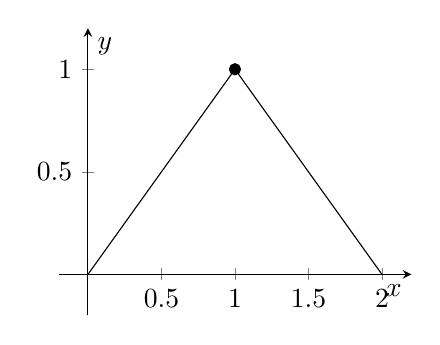
\begin{tikzpicture}
\begin{axis}[xmax = 2.2, xmin = -0.2, ymax = 1.2, ymin = -0.2,
             axis lines=middle, xlabel=$x$, ylabel=$y$,
             xtick={0, 0.5, 1, 1.5, 2},
             ytick={0.5, 1},
             xlabel style={anchor=north east},
             xticklabel style={anchor=north},
             yticklabel style={anchor=east},
             width=0.5\linewidth,
            ]
	\addplot[domain=0:1, samples=200]{x};
	\addplot[domain=1:2, samples=200]{2-x};
\addplot [only marks, mark options={scale=1}] table {
1 1
};
\end{axis}
\end{tikzpicture}
	\caption{Caso di una funzione non derivabile nel teorema di Rolle}
	\label{fig_esempioRolle}

\end{figure}


\subsubsection{Teorema di Lagrange} \label{sec_teoremaLagrange}
\thm {
Data una funzione $f:[a,b] \to \mathbb{R}$ con le seguenti proprietà:
\begin{enumerate}
    \item $f$ è continua su $[a,b]$
    \item $f$ è derivabile su $]a,b[$
\end{enumerate}
Allora:
\begin{equation*}
    \exists \,c \in ]a,b[ \;: \dfrac{f(b)-f(a)}{b-a} = f'(c)
\end{equation*}
}
Un esempio grafico di questo teorema è quello riportato in figura 
\ref{fig_teoremaLagrange}. Il termine:
\begin{equation*}
	\dfrac{f(b)-f(a)}{b-a}
\end{equation*}
può essere considerato come la pendenza media del percorso (che in questo caso 
è la funzione) tra il punto $a$ e il punto $b$. Esiste quindi, per questo 
teorema, un ulteriore punto in cui la tangente sarà esattamente come questa 
pendenza media. 

\begin{figure}[h]
\centering
\begin{tikzpicture}
\begin{axis}[xmax = 10, xmin = -0.2, ymax = 3.5, ymin = -0.2,
             axis lines=middle, xlabel=$x$, ylabel=$y$,
             xtick={2.53, 4.67, 7},
             ytick={1, 3},
	     xticklabels={$a$, $c$, $b$},
	     yticklabels={$f(a)$, $f(b)$},
             xlabel style={anchor=north east},
             xticklabel style={anchor=north},
             yticklabel style={anchor=east},
             width=0.7\linewidth,
            ]
	\addplot[domain=0:10, samples=200]{-0.1 * (x-7) * (x-7) + 3};
	\addplot[domain=1:10, samples=200]{(2*x -0.57) / 4.47};
	\addplot[domain=1:10, samples=200, dashed]{(2*x +1.66) / 4.47};
	\addplot[domain=2.53:7, samples=200, dotted]{1};
	\addplot +[mark=none, dotted, black] coordinates {(7, 1) (7, 3)};
\addplot [only marks, mark options={scale=1}] table {
2.53 1
4.67 2.46
7 3
};
\end{axis}
\end{tikzpicture}
	\caption{Caso di una funzione non derivabile nel teorema di Rolle}
	\label{fig_teoremaLagrange}
\end{figure}

\pf{
	Per provare questo teorema è necessario utilizzare il teorema di Rolle 
    (Sezione: \ref{sec_teoremaRolle}). Purtroppo si tende a creare molta 
    confusione tra questi teoremi perché si può vedere questo come 
    un'estensione del teorema di Rolle e quindi la dimostrazione di 
    quest'ultimo si potrebbe fare a partire da questo. Ma come già detto il 
    teorema di Lagrange si basa proprio sul teorema di Rolle, quindi nonostante 
    possa essere visto come una generalizzazione, il teorema di Rolle non può 
    essere provato a partire da questo teorema.\\

	Dobbiamo dimostrare il teorema di Lagrange. Prendiamo una funzione $f:[a,b] 
    \to \mathbb{R}$ e assumiamo le seguenti proprietà come ipotesi:
	\begin{enumerate}
	    \item $f$ è continua su $[a,b]$
	    \item $f$ è derivabile su $]a,b[$
	\end{enumerate}
	Scegliamo una funzione ausiliaria $g:[a, b] \to \mathbb{R}$ tale che:
	\begin{equation*}
		g(x) = f(x) + k \cdot x \qquad (k \in \mathbb{R})
	\end{equation*}
	Da ipotesi 1 $g$ è continua su $[a, b]$ perché è fatta da una somma di 
    funzioni continue e da ipotesi 2 $g$ è derivabile su $]a,b[$ perché è fatta 
    da somma di funzioni derivabili.

	Vogliamo scegliere $k \in \mathbb{R}$ in modo che si possa applicare il 
    teorema di Rolle: 
	\begin{align*}
		g(a) &= f(a) + k \cdot a \\[10pt]
		g(b) &= f(b) + k \cdot b
	\end{align*}
	Scegliamo quindi $k$ in modo che:
	\begin{align*}
		g(a) &= g(b)\\[10pt]
		f(a) + k \cdot a &= f(b) + k \cdot b\\[10pt]
		k (b - a) &= f(a) - f(b)\\[10pt]
		k &= \dfrac{f(a) - f(b)}{b-a}
	\end{align*}
	Dal teorema di Rolle:
	\begin{equation*}
		\exists c \in ]a, b[ : g'(c) = 0
	\end{equation*}
	Quindi:
	\begin{equation*}
		g'(c) = 0 \implies f'(c) + k = 0
	\end{equation*}
	E infine:
	\begin{equation*}
		f'(c) = -k = \dfrac{f(b)-f(a)}{b-a}
	\end{equation*}
}

\imp{
    \textbf{Corollario}: se una funzione $f:]a, b[ \to \mathbb{R}$, continua e 
    derivabile su $]a, b[$ ha derivata sempre zero per tutti i punti del 
    dominio, allora la funzione è costante.
}

\pf{
	Dimostriamo il corollario: prendiamo una funzione $f:]a,b[ \to \mathbb{R}$ 
    in modo che sia costante, continua e derivabile in $]a,b[$. Assumiamo che 
    la sua derivata sia sempre 0. Se prendiamo due punti casuali 
    nell'intervallo $]a, b[$:
	\begin{equation*}
		\forall x_1, x_2 \in ]a, b[ : x_1 < x_2
	\end{equation*}
	Si può applicare il teorema di Lagrange alla funzione (in quanto $[x1, x2] 
    \subseteq ]a, b[$ e quindi la funzione rispetta tutte le premesse del 
    teorema):
	\begin{equation*}
		f:[x_1, x_2] \to \mathbb{R}
	\end{equation*}
	Dal teorema quindi:
	\begin{equation*}
		\exists c \in ]x_1, x_2[ : \dfrac{f(x_2) - f(x_1)}{x_2 - x_1} = f'(c) 
        = 0
	\end{equation*}
	Dall'ipotesi $f'(c)$ è sempre 0, e quindi:
	\begin{equation*}
		f(x_2) = f(x_1) \qquad \forall x_1, x_2 \in ]a,b[
	\end{equation*}
	\hfill Qed.
}
Le ipotesi del corollario sono importanti perché se non vengono rispettate non 
funzione più. Prendiamo come esempio la funzione
\begin{equation*}
	f(x) = \arctan{x} + \arctan{\dfrac{1}{x}}
\end{equation*}
La sua derivata sarà:
\begin{align*}
	f'(x) &= \dfrac{1}{1+x^2} + \dfrac{1}{1+\left( \dfrac{1}{x}\right)^2} \cdot 
    \left( -\dfrac{1}{x^2}\right) = \dfrac{1}{1+x^2} - \dfrac{1}{\left(1 + 
    \dfrac{1}{x^2}\right) \cdot x^2} = \dfrac{1}{1+x^2} - \dfrac{1}{x^2 + 1} 
    = 0
\end{align*}
Tuttavia:
\begin{align*}
	f(-1) &= \arctan(-1) + \arctan \left(\dfrac{1}{-1}\right) = 
    -\dfrac{\pi}{2}\\[10pt]
	f(1) &= \arctan(1) + \arctan \left(\dfrac{1}{1}\right) = \dfrac{\pi}{2}
\end{align*}
Non vi è in realtà contraddizione con il corollario perché il dominio di $f$ è 
$\mathbb{R} \setminus \{0\}$, che non è un intervallo. La funzione è 
effettivamente costante sia a destra che a sinistra di 0, ma la costante è 
diversa. Il grafico infatti risulta come da figura 
\ref{fig_esempioCorollarioLagrange}.

\begin{figure}[h]
\centering
\begin{tikzpicture}
\begin{axis}[xmax = 2, xmin = -2, ymax = 1.5, ymin = -1.5,
             axis lines=middle, xlabel=$x$, ylabel=$y$,
             xtick={100},
             ytick={-1, 1},
	     yticklabels={-1, 1},
             xlabel style={anchor=north east},
             xticklabel style={anchor=north},
             yticklabel style={anchor=south west},
             width=0.7\linewidth,
            ]
	\addplot[domain=0:3, samples=200]{1};
	\addplot[domain=-3:0, samples=200]{-1};
\addplot [only marks, mark options={scale=1.2}] table {
0 1
0 -1
};
\addplot [only marks, mark options={scale=1}, white] table {
0 1
0 -1
};
\end{axis}
\end{tikzpicture}
	\caption{Caso di una funzione che non ha il dominio in un intervallo nel 
    corollario di Lagrange}
	\label{fig_esempioCorollarioLagrange}
\end{figure}


\subsubsection{Teorema di Cauchy} \label{sec_teoremaCauchy}
\thm {
Date due funzioni $f,g:[a,b] \to \mathbb{R}$ con le seguenti proprietà:
\begin{enumerate}
    \item $f,g$ è continue su $[a,b]$
    \item $f,g$ è derivabili su $]a,b[$
    \item $g'(x) \neq 0 \quad \forall x\in ]a,b[$
\end{enumerate}
Allora:
\begin{equation*}
    \exists \,c \in ]a,b[ \;: \dfrac{f(b)-f(a)}{g(b)-g(a)} = 
    \dfrac{f'(c)}{g'(c)}
\end{equation*}
}
La condizione che $g(b) - g(a) \neq 0$ è intrinseca alla premessa numero 3. Se 
infatti fosse che $g(b) - g(a) = 0$ diventerebbe $g(b) = g(a)$ che in 
combinazione con le premesse 1 e 2 del teorema permetterebbe l'applicazione 
del teorema di Rolle (Sezione: \ref{sec_teoremaRolle}) e quindi $\exists d \in 
]a,b[ : g'(d) = 0$ che è in contraddizione con l'ipotesi numero 3.

Per la dimostrazione si potrebbe pensare erroneamente che applicando il 
teorema di Lagrange prima al numeratore e poi al denominatore si possa 
dimostrare questo teorema. Le premesse ci permettono di applicare Lagrange, ma 
nessuno ci assicura che il punto in cui si annulla $f'$ è lo stesso punto in 
cui si annulla $g'$:
\begin{equation*}
	\dfrac{f(b) - f(a)}{g(b) - g(a)} = \dfrac{\dfrac{f(b) - f(a)}{b-a}}
    {\dfrac{g(b)-g(a)}{b - a}} = \dfrac{f'(c_1)}{g'(c_2)}
\end{equation*}
Nessuno infatti ci assicura che $c_1 = c_2$, risulta quindi necessario fare una 
dimostrazione a parte:

\pf{
	Dobbiamo dimostrare il teorema di Cauchy. Prendiamo due funzioni $f,g:[a,b] 
    \to \mathbb{R}$ e assumiamo le seguenti proprietà come ipotesi:
	\begin{enumerate}
	    \item $f,g$ è continue su $[a,b]$
	    \item $f,g$ è derivabili su $]a,b[$
	    \item $g'(x) \neq 0 \quad \forall x\in ]a,b[$
	\end{enumerate}
	Consideriamo ora una funzione ausiliaria $h:[a, b] \to \mathbb{R}$:
	\begin{equation*}
		h(x) = f(x) + k \cdot g(x) \qquad (k \in \mathbb{R})
	\end{equation*}
	Per ipotesi 1 e 2 $h$ è continua su $[a, b]$ e derivabile su $]a, b[$. 
    Vogliamo applicare il teorema di teorema di Rolle ad $h$: 
	\begin{align*}
		h(a) &= f(a) + k \cdot g(a) \\[10pt]
		h(b) &= f(b) + k \cdot g(b)
	\end{align*}
	Dobbiamo quindi scegliere $k$ in modo che:
	\begin{align*}
		h(a) &= h(b)\\[10pt]
		f(a) + k \cdot g(a) &= f(b) + k \cdot g(b) \\[10pt]
		f(b) - f(a) &= k (g(a) - g(b))
	\end{align*}
	Per ipotesi 3 so che $g(a) - g(b) \neq 0$, quindi posso dividere:
	\begin{equation*}
		k = \dfrac{f(b) - f(a)}{g(a) - g(b)}
	\end{equation*}
	Applichiamo quindi il teorema di Rolle ad $h$:
	\begin{equation*}
		\exists c \in ]a, b[ : h'(c) = 0
	\end{equation*}
	Cioè:
	\begin{align*}
		h'(c) &= f'(c) + k \cdot g'(c) = 0\\[10pt]
		f'(c) &= -k \cdot g'(c)
	\end{align*}
	E quindi:
	\begin{equation*}
	    \dfrac{f'(c)}{g'(c)} = -k = \dfrac{f(b)-f(a)}{g(b)-g(a)}
	\end{equation*}
	\hfill Qed.
}

\subsubsection{Legame tra derivata e monotonia di una funzione}
Questo teorema è fondamentale nello studio di funzione perché permette. in base 
al segno della derivata, di determinare la monotonia della funzione in esame.
\thm{
	Data una funzione $f:]a,b[ \to \mathbb{R}$ se è derivabile su $]a,b[$ 
    allora:
	\begin{enumerate}
		\item 
			\begin{equation*}
				f'(x) \geq 0 \quad \forall x \in ]a,b[ \iff f \; \text{è 
                crescente su } ]a,b[
			\end{equation*}

			Vale anche per il caso $\leq$:
			\begin{equation*}
				f'(x) \leq 0 \quad \forall x \in ]a,b[ \iff f \; \text{è 
            decrescente su } ]a,b[
			\end{equation*}

		\item
			\begin{equation*}
				f'(x) > 0 \quad \forall x \in ]a,b[ \implies f \; \text{è 
            strettamente crescente su } ]a,b[
			\end{equation*}

			Vale anche il caso $<$:
			\begin{equation*}
				f'(x) < 0 \quad \forall x \in ]a,b[ \implies f \; \text{è 
            strettamente decrescente su } ]a,b[
			\end{equation*}
	\end{enumerate}
}
Nei casi 2 e 3 non vale l'implicazione contraria perché alcune funzioni 
strettamente crescenti o strettamente decrescenti possono avere anche derivata 
nulla in un punto, tipo $x^3$ e $-x^3$ in $x = 0$.

\pf{
	Prendiamo una funzione $f:]a,b[ \to \mathbb{R}$ e assumiamo come ipotesi 
che sia derivabile su $]a,b[$. 
	\begin{enumerate}
		\item Caso $\implies$: Dobbiamo provare che:
			\begin{equation*}
				f'(x) \geq 0 \quad \forall x \in ]a,b[ \implies f \; \text{è 
                crescente su } ]a,b[
			\end{equation*}
			Assumiamo come ipotesi che  $f'(x) \geq 0 \; \forall x \in ]a,b[$ 
        per dimostrare che:
			\begin{equation*}
				f \; \text{è crescente su } ]a,b[
			\end{equation*}
			In pratica dobbiamo provare che:
			\begin{equation*}
				\forall x_1, x_2 \in ]a,b[ : x_1 < x_2 \implies f(x_1) \leq 
                f(x_2)
			\end{equation*}
			Applichiamo il teorema di Lagrange (Sezione: 
            \ref{sec_teoremaLagrange}) alla funzione $f:[x_1, x_2] \to 
            \mathbb{R}$ con il dominio quindi ristretto a $[x_1, x_2]$:
			\begin{equation*}
				\exists c \in ]x_1, x_2[ \; : \; \dfrac{f(x_2) - f(x_1)}{x_2 - 
                x_1} = f'(c)
			\end{equation*}
			Per ipotesi $f'(c) \geq 0$ ed essendo sempre per ipotesi $x_2 - 
            x_1 > 0$:
			\begin{align*}
				f(x_2) &- f(x_1) \geq 0\\[10pt]
				f(x_2) &\geq f(x_1)
			\end{align*}
			Quindi abbiamo concluso questo caso. Nel caso del $\leq$ si fa 
            uguale.\\

			Caso $\impliedby$: In questo caso l'uso diretto del teorema di 
            Lagrange non permette di concludere quello che vogliamo dimostrare, 
            infatti non riuscirei a dimostrare la cosa per tutti i punti. 
            Dobbiamo provare che:
			\begin{equation*}
				f \; \text{è una funzione crescente su } ]a,b[ \implies 
                \forall x \in ]a, b[ \; f'(x) \geq 0 
			\end{equation*}
			Assumiamo che $f$ sia crescente su $]a,b[$ per dimostrare:
			\begin{equation*}
				f'(x) \geq 0 \quad \forall x \in ]a, b[
			\end{equation*}
			Essendo crescente:
			\begin{equation*}
				\forall x_0 \in ]a,b[ : x > x_0 \implies f(x) \geq f(x_0)
			\end{equation*}
			Visto che $x - x_0 > 0$ e $f(x) - f(x_0) \geq 0$, ne consegue:
			\begin{equation*}
				\dfrac{f(x) - f(x_0)}{x - x_0} \geq 0
			\end{equation*}
			Essendo per ipotesi derivabile e dal teorema di permanenza del 
            segno (Sezione: \ref{theorem_permanenzaSegno}):
			\begin{equation*}
				f'(x_0) = \lim_{x \to x_0} \dfrac{f(x) - f(x_0)}{x - x_0} 
                \geq 0
			\end{equation*}
			E questo vale $\forall x_0 \in ]a,b[$, quindi abbiamo finito.

		\item Questo caso si fa esattamente come il punto 1, ma lo riporto lo 
            stesso. Dobbiamo provare che:
			\begin{equation*}
				f'(x) > 0 \quad \forall x \in ]a,b[ \implies f \; \text{è 
                strettamente crescente su } ]a,b[
			\end{equation*}
			Assumiamo come ipotesi che  $f'(x) > 0 \; \forall x \in ]a,b[$ 
        per dimostrare che:
			\begin{equation*}
				f \; \text{è strettamente crescente su } ]a,b[
			\end{equation*}
			In pratica dobbiamo provare che:
			\begin{equation*}
				\forall x_1, x_2 \in ]a,b[ : x_1 < x_2 \implies f(x_1) < f(x_2)
			\end{equation*}
			Applichiamo il teorema di Lagrange (Sezione: 
            \ref{sec_teoremaLagrange}) alla funzione $f:[x_1, x_2] \to 
            \mathbb{R}$:
			\begin{equation*}
				\exists c \in ]x_1, x_2[ \; : \; \dfrac{f(x_2) - f(x_1)}{x_2 - 
                x_1} = f'(c)
			\end{equation*}
			Per ipotesi $f'(c) > 0$ ed essendo sempre per ipotesi $x_2 - x_1 > 
            0$:
			\begin{align*}
				f(x_2) &- f(x_1) > 0\\[10pt]
				f(x_2) &> f(x_1)
			\end{align*}
			Quindi abbiamo concluso questo caso. Nel caso del $<$ si fa 
            uguale.\\
	\end{enumerate}
	\hfill Qed.
}

\textbf{Proposizione:} Data una funzione $f:]a,b[ \to \mathbb{R}$ che sia 
derivabile su $]a,b[$ se vale che:
\begin{enumerate}
	\item $f'(x) \geq 0 \quad \forall x \in ]a,b[$ 
	
	\item Posto $N = \{x \in ]a,b[ \; | \; f'(x) = 0\}$, $N$ è un insieme 
        finito.
\end{enumerate}
Allora:
\begin{center}
	$f$ è strettamente crescente
\end{center}
Vale anche per il caso in cui $f'(x) \leq 0 \; \forall x \in ]a,b[$, che però 
rende la funzione \textit{strettamente decrescente}.

\pf{
	Dobbiamo dimostrare la proposizione appena enunciata. Prendiamo una 
    funzione $f:]a,b[ \to \mathbb{R}$ che sia derivabile su $]a,b[$. Assumiamo 
    come ipotesi che valgono le seguenti proprietà:
	\begin{enumerate}
		\item $f'(x) \geq 0 \quad \forall x \in ]a,b[$ 
		
		\item Posto $N = \{x \in ]a,b[ \; | \; f'(x) = 0\}$, $N$ è un insieme 
            finito.
	\end{enumerate}
	Dalla prima ipotesi e dal teorema appena enunciato:
	\begin{center}
		$f$ è crescente su $]a,b[$
	\end{center}
	Assumiamo come ipotesi che $f$ NON sia strettamente crescente e riduciamoci 
    a dimostrare l'assurdo\footnote{RAAAAAAA}. Essendo per che $f$ non è 
    strettamente crescente:
	\begin{equation*}
		\exists x_1, x_2 \in ]a, b[ \; : \; x_1 < x_2 \land f(x_1) = f(x_2)
	\end{equation*}
	Siccome però $f$ è crescente:
	\begin{equation*}
		\forall x \in ]x_1, x_2[ \; : \; f(x_1) \leq f(x) \leq f(x_2)
	\end{equation*}
	Ma essendo $f(x_1) = f(x_2)$:
	\begin{center}
		$f$ è costante su $[x_1, x_2]$
	\end{center}
	Di conseguenza:
	\begin{equation*}
		f'(x) = 0 \quad \forall ]x_1, x_2[
	\end{equation*}
	Che però è in contraddizione con l'ipotesi 2. Usando quindi una 
    \textit{not eliminazione}\footnote{Deduzione naturale insegna} abbiamo 
    provato l'assurdo!
	\hfill Qed.
}


\subsubsection{I teoremi di De L'Hôpital} \label{sec_deLHopital}

Per dimostrare i teoremi di De L'Hôpital è necessario il seguente lemma che 
"traduce" la nozione di limite usando le successioni:
\mlem{
	Data una funzione $h: A \to \mathbb{R}$ e un punto $x_0 \in \mathcal{D}(A)$ 
    allora: %non sono sicuro di cosa sia D
	\begin{equation*}
        l \in \mathbb{R} \cup \{+\infty\} \cup \{-\infty\}
	\end{equation*}
	\begin{enumerate}
		\item 
			\begin{equation*}
				\lim_{x \to x_0^-} h(x) = l \iff \forall (x_n)_n \subseteq A, 
                \, x_n < x_0 \;\; \forall n \; \text{tale che: } x_n 
                \xrightarrow[n \to + \infty]{} x_0 \; \text{si ha: } h(x_n) 
                \xrightarrow[n \to +\infty]{} l
			\end{equation*}
		\item 
			\begin{equation*}
				\lim_{x \to x_0^+} h(x) = l \iff \forall (x_n)_n \subseteq A, 
                \, x_n > x_0 \;\; \forall n \; \text{tale che: } x_n 
                \xrightarrow[n \to + \infty]{} x_0 \; \text{si ha: } h(x_n) 
                \xrightarrow[n \to +\infty]{} l
			\end{equation*}
	\end{enumerate}
	Senza dimostrazione da 1 e 2 segue che:
	\begin{enumerate}
		\setcounter{enumi}{2} %mi serve per fare  partire la lista da 3
		\item  
			\begin{equation*}
				\lim_{x \to x_0} h(x) = l \iff \forall (x_n)_n \subseteq A, 
                \, x_n \neq x_0 \;\; \forall n \; \text{tale che: } x_n 
                \xrightarrow[n \to + \infty]{} x_0 \; \text{si ha: } h(x_n) 
                \xrightarrow[n \to +\infty]{} l
			\end{equation*}
	\end{enumerate}
}

Da qui nasce un criterio per mostrare che non esiste il limite per un punto di 
una funzione. Cioè se voglio far vedere che:
\begin{equation*}
	\not \exists \lim_{x \to x_0} h(x)
\end{equation*}
Mi basta trovare due successioni che tendono entrambe ad $x_0$:
\begin{align*}
	x_n \xrightarrow[n \to + \infty]{} x_0\\
	y_n \xrightarrow[n \to + \infty]{} x_0\\
\end{align*}
E poi calcolare il loro limite e far vedere che i valori non coincidono. Di 
conseguenza il limite non esiste perché non è unico.
\begin{gather*}
	h(x_n) \xrightarrow[n \to +\infty]{} l1\\
	h(y_n) \xrightarrow[n \to +\infty]{} l2\\
	l1 \neq l2
\end{gather*}

\thm{
	\textbf{Caso 1 limite al finito}: Preso un intervallo $I \subseteq{R}$ e un 
    punto $x_0 \in \mathring{I}$ se:
	\begin{enumerate}
		\item Due funzioni $f, g: I \to \mathbb{R}$ continue su I e con 
            $f(x_0) = g(x_0) = 0$

		\item $f, g$ derivabili in $I \setminus \{x_0\}$ e $g'(x) \neq 0$ se 
            $x \in I \setminus \{x_0\}$

		\item 
			\begin{equation*}
				\exists \lim_{x \to x_0} \dfrac{f'(x)}{g'(x)} = l \in 
                \mathbb{R} \cup \{+\infty\} \cup \{-\infty\}
			\end{equation*}
	\end{enumerate}
	Allora:
	\begin{equation*}
		\exists \lim_{x \to x_0} \dfrac{f(x)}{g(x)} = \lim_{x \to x_0} 
        \dfrac{f'(x)}{g'(x)} 
	\end{equation*}
}
Alcune considerazioni importanti da fare:
\begin{itemize}
	\item Non serve specificare che $g(x) \neq 0$ se $x \in I\setminus \{x_0\}$ 
        perché è già intrinseco nella seconda ipotesi del teorema. Supponiamo 
        infatti che:
		\begin{equation*}
			\exists x_1 \in I : x_1 \neq x_0 \land g(x_1) = 0
		\end{equation*}
		La funzione $g:[x_0, x_1] \to \mathbb{R}$ è continua su $[x_0, x_1]$, è 
        derivabile in $]x_0,x_1[$ e inoltre, per quanto appena assunto e per la 
        prima ipotesi del teorema, $g(x_0) = 0 = g(x_1)$. Ne consegue che dal 
        teorema di Rolle (Sezione: \ref{sec_teoremaRolle}):
		\begin{equation*}
			\exists x \in ]x_0, x_1[ \; : \; g'(c) = 0
		\end{equation*}
		Che però è in contrasto con la seconda ipotesi del teorema.

	\item È estremamente importante la direzione dell'implicazione: se esiste 
        il limite del rapporto delle derivate allora esiste il limite del 
        rapporto delle funzioni ed è uguale al limite del rapporto delle 
        derivate. Se però il limite delle derivate non esiste, il teorema non 
        si può applicare. Nessuno però ci dice il limite in sé non esista. Non 
        vale quindi il contrario. Se esiste il limite di un rapporto di 
        funzioni non è detto che esista il limite del rapporto delle derivate.

		Consideriamo le funzioni:
		\begin{align*}
			&f(x) = 
			\begin{cases*}
				x^2 \cdot \sin{\dfrac{1}{x}} \quad \text{se } x \neq 0\\
				0 \qquad \qquad \;\; \text{se } x = 0
			\end{cases*}\\[10pt]
			&g(x) = x
		\end{align*}
		Facciamo vedere che:
		\begin{equation*}
			\not \exists \lim_{x \to 0} \dfrac{f'(x)}{g'(x)}
		\end{equation*}
		Ma che tuttavia:
		\begin{equation*}
			\exists \lim_{x \to 0} \dfrac{f(x)}{g(x)}
		\end{equation*}
		Se infatti sostituiamo le funzioni con la loro definizione:
		\begin{equation*}
			\lim_{x \to 0} \dfrac{f(x)}{g(x)} = \lim_{x \to 0} \dfrac{x^2 \cdot 
            \sin{\dfrac{1}{x}}}{x} = \lim_{x \to 0} x \cdot \sin{\dfrac{1}{x}} 
            = 0
		\end{equation*}
		Fa 0 in quanto $x \to 0$ e :
		\begin{equation*}
			0 \leq \left| x \cdot \sin{\dfrac{1}{x}} \right| \leq |x|
		\end{equation*}
		Proviamo ora a calcolare il limite delle derivate assumendo che $x 
        \neq 0$. Calcoliamo prima le derivate delle funzioni singolarmente:
		\begin{equation*}
			f'(x) = 2x \cdot \sin \left(\dfrac{1}{x} \right) + x^2 \cdot \cos 
            \left(\dfrac{1}{x} \right) \cdot -\dfrac{1}{x^2} = 2x \cdot \sin 
            \left(\dfrac{1}{x} \right) + \cos \left(\dfrac{1}{x} \right) 
		\end{equation*}
		\begin{equation*}
			g'(x) = 1
		\end{equation*}
		Ne consegue che:
		\begin{equation*}
			\lim_{x \to 0} \dfrac{f'(x)}{g'(x)} = \lim_{x \to 0} 2x \cdot \sin 
            \left(\dfrac{1}{x} \right) + \cos \left(\dfrac{1}{x} \right) 
		\end{equation*}
		Il termine $2x \cdot \sin \left(\frac{1}{x} \right)$ va a 0 come 
        abbiamo già visto, mentre il termine $\cos \left(\frac{1}{x} \right)$ 
        non ha limite (dimostrato dopo). Ne consegue che non esiste il limite 
        del rapporto delle derivate nonostante il limite del rapporto delle 
        funzioni esiste. Per completezza il grafico del rapporto delle funzioni 
        e rappresentato in figura \ref{fig_esempioDeLHopital1}.

	\begin{figure}[h]
	\centering
	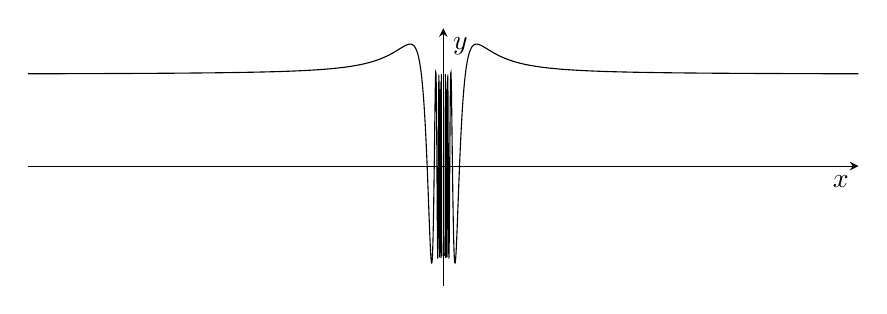
\begin{tikzpicture}
	\begin{axis}[xmax = 6, xmin = -6, ymax = 1.5, ymin = -1.3,
		     axis lines=middle, xlabel=$x$, ylabel=$y$,
		     xtick={10},
		     ytick={10},
		     xlabel style={anchor=north east},
		     xticklabel style={anchor=north},
		     yticklabel style={anchor=east},
		     width=\linewidth,
		     height=0.4\linewidth
		    ]
		\addplot[domain=-6:-0.02, samples=2000]{2 * x * sin(deg(1/x)) - 
            cos(deg(1/x))};
		\addplot[domain=0.02:6, samples=2000]{2 * x * sin(deg(1/x)) - 
            cos(deg(1/x))};
	\end{axis}
	\end{tikzpicture}
		\caption{Grafico di $2x \cdot \sin(\dfrac{1}{x}) - \cos(\dfrac{1}{x})$}
		\label{fig_esempioDeLHopital1}
	\end{figure}

	Per mostrare che:
	\begin{equation*}
		\not \exists \lim_{x \to 0} \cos \left(\dfrac{1}{x}\right)
	\end{equation*}
	Usiamo il lemma enunciato qualche pagina sopra. Assumiamo che esiste il 
    limite (chiamiamo il suo valore $l$) e riduciamoci a dimostrare l'assurdo. 
    Dal lemma:
	\begin{equation*}
		\forall (x_n)_n \subseteq A, \, x_n \geq x_0 \;\; \forall n \; 
        \text{tale che: } x_n \xrightarrow[n \to + \infty]{} x_0 \; 
        \text{si ha: } h(x_n) \xrightarrow[n \to +\infty]{} l
	\end{equation*}
	Ora mostreremo che esistono due successioni tali che tendono entrambe a 
    $0$ ma sulla funzione hanno limiti diversi. La prima successione:
	\begin{equation*}
		x_n = \dfrac{1}{2 \pi \cdot n} \;\; \xrightarrow[n \to +\infty]{} 0
	\end{equation*}
	Se calcoliamo il limite della funzione:
	\begin{equation*}
		\lim_{n \to +\infty} \cos \left(\dfrac{1}{x_n}\right) = \lim_{n \to 
        +\infty} \cos \left(\dfrac{1}{\dfrac{1}{2 \pi \cdot n}}\right) = 
        \lim_{n \to +\infty} \cos(2\pi \cdot n) = 1
	\end{equation*}
	Questo perché $n \in \mathbb{N}$ facendo parte di una successione è per 
    forza un numero intero. Ne consegue che anche se tende a $+\infty$ 
    l'argomento del coseno avrà sempre multipli interi di $2\pi$, e di 
    conseguenza farà sempre 1\footnote{Questa è una mia interpretazione perché 
    sugli appunti non è specificato e non si capisce come faccia a fare 1, 
    però mi sembra l'unica con un minimo di senso}. Prendiamo ora la seconda 
    successione:
	\begin{equation*}
		y_n = \dfrac{1}{\dfrac{\pi}{2} \cdot 2\pi \cdot n} \;\; \xrightarrow[n 
        \to +\infty]{} 0
	\end{equation*}
	Calcolando il limite e notando sempre che $n \in \mathbb{N}$:
	\begin{equation*}
		\lim_{n \to +\infty} \cos \left( \dfrac{1}{y_n} \right) = \lim_{n \to 
        +\infty} \left(  \dfrac{1}{\dfrac{\pi}{2} \cdot 2\pi \cdot n} \right) = 
        \lim_{n \to +\infty} \cos \left( \dfrac{\pi}{2} \cdot 2\pi \cdot n 
        \right) = 0
	\end{equation*}
	Visto quindi che i due limiti non sono uguali segue che:
	\begin{equation*}
        \not \exists \lim_{x \to 0^+} \cos(\dfrac{1}{x}) 
	\end{equation*}
	E quindi:
	\begin{equation*}
        \not \exists \lim_{x \to 0} \cos(\dfrac{1}{x}) 
	\end{equation*}


\end{itemize}

Dimostriamo ora il teorema:

\pf{
	Dobbiamo dimostrare il teorema appena enunciato. Prendiamo un intervallo 
    $I \subseteq \mathbb{R}$ e un punto $x_0 \in \mathring{I}$. Assumiamo 
    inoltre le seguenti ipotesi:
	\begin{enumerate}
		\item Due funzioni $f, g: I \to \mathbb{R}$ continue su I e con $f(x_0) 
            = g(x_0) = 0$

		\item $f, g$ derivabili in $I \setminus \{x_0\}$ e $g'(x) \neq 0$ se 
            $x \in I \setminus \{x_0\}$

		\item 
			\begin{equation*}
				\exists \lim_{x \to x_0} \dfrac{f'(x)}{g'(x)} = l \in 
                \mathbb{R} \cup \{+\infty\} \cup \{-\infty\}
			\end{equation*}
	\end{enumerate}
	Dobbiamo provare che:
	\begin{equation*}
		\exists \lim_{x \to x_0} \dfrac{f(x)}{g(x)} = \lim_{x \to x_0} 
        \dfrac{f'(x)}{g'(x)} 
	\end{equation*}
	In altre parole:
	\begin{equation*}
		\exists \lim_{x \to x_0^-} \dfrac{f(x)}{g(x)} = l \quad \land \quad 
        \exists \lim_{x \to x_0^+} \dfrac{f(x)}{g(x)} = l
	\end{equation*}
	Proviamo solo uno dei due tanto l'altro è analogo. Scegliamo quindi di 
    provare:
	\begin{equation*}
		\exists \lim_{x \to x_0^+} \dfrac{f(x)}{g(x)} = l
	\end{equation*}
	A tal fine, usiamo il lemma precedente: ci riduciamo quindi a provare:
	\begin{equation*}
		\forall (x_n)_n \subseteq A, \, x_n > x_0 \;\; \forall n \; \text{tale 
        che: } x_n \xrightarrow[n \to + \infty]{} x_0 \; \text{si ha: } 
        \lim_{n \to + \infty} \dfrac{f(x_n)}{g(x_n)} = l
	\end{equation*}	
	Assumiamo le premesse per dimostrare che:
	\begin{equation*}
		\lim_{n \to + \infty} \dfrac{f(x_n)}{g(x_n)} = l
	\end{equation*}	
	Per ipotesi 1 $f(x_0) = g(x_0) = 0$. Di conseguenza, in quanto nulli, 
    possiamo sommarli e sottrarli a piacere:
	\begin{equation*}
		\dfrac{f(x_n)}{g(x_n)} = \dfrac{f(x_n) - f(x_0)}{g(x_n) - g(x_0)}
	\end{equation*}
	Se ora restringiamo il dominio alle funzioni $f,g:[x_0, x_n] \to 
    \mathbb{R}$ possiamo applicare il teorema di Cauchy (Sezione: 
    \ref{sec_teoremaCauchy}):
	\begin{equation*}
		\exists c_n \in ]x_0, x_n[ \;\; \text{tale che } \;\; \dfrac{f(x_n) - 
        f(x_0)}{g(x_n) - g(x_0)} = \dfrac{f'(c_n)}{g'(c_n)}
	\end{equation*}
	Essendo $c_n$ "intrappolata" tra $x_0$ e $x_n$:
	\begin{equation*}
		x_0 < c_n < x_n
	\end{equation*}
	Ed essendo per ipotesi:
	\begin{equation*}
		x_n \xrightarrow[n \to + \infty]{} x_0
	\end{equation*}
	Ne consegue che:
	\begin{equation*}
		c_n \xrightarrow[n \to + \infty]{} x_0
	\end{equation*}
	Dall'ipotesi 3 del teorema:
	\begin{equation*}
		\lim_{x \to x_0^+} \dfrac{f'(x)}{g'(x)} = l
	\end{equation*}
	Dunque dal lemma (ricordiamoci che $c_n \to x_0$ e che $x_0 < c_n$):
	\begin{equation*}
		\lim_{n \to +\infty} \dfrac{f'(c_n)}{g'(c_n)} = l
	\end{equation*}
	Ricapitolando:
	\begin{equation*}
		\dfrac{f(x_n)}{g(x_n)} = \dfrac{f(x_n) - f(x_0)}{g(x_n) - g(x_0)} = 
        \dfrac{f'(c_n)}{g'(c_n)}
	\end{equation*}
	Quindi:
	\begin{equation*}
		\lim_{n \to + \infty} \dfrac{f(x_n)}{g(x_n)} = l
	\end{equation*}
	Dal lemma:
	\begin{equation*}
		\lim_{x \to x_0^+} \dfrac{f(x)}{g(x)} = l = \lim_{x \to x_0} 
        \dfrac{f'(x)}{g'(x)}
	\end{equation*}
	Analogamente si prova che:
	\begin{equation*}
		\lim_{x \to x_0^-} \dfrac{f(x)}{g(x)} = l = \lim_{x \to x_0} 
        \dfrac{f'(x)}{g'(x)}
	\end{equation*}
	Da cui:
	\begin{equation*}
		\lim_{x \to x_0} \dfrac{f(x)}{g(x)} = \lim_{x \to x_0} 
        \dfrac{f'(x)}{g'(x)}
	\end{equation*}
	\hfill Qed.
}
Dei seguenti teoremi non vi è la dimostrazione:

\thm{ 
	\textbf{Caso 2 limite al finito}: Prese due funzioni $f, g:]a,b[ \to 
    \mathbb{R}$ derivabili:
	\begin{enumerate}
		\item
			\begin{equation*}
				\lim_{x \to x_0} f(x) = \lim_{x \to x_0} g(x) = \pm \infty 
			\end{equation*}

		\item 
			\begin{equation*}
				g'(x) \neq 0 \;\; \forall x \in ]a,b[ \; \setminus \{x_0\}
			\end{equation*}

		\item 
			\begin{equation*}
				\exists \lim_{x \to x_0} \dfrac{f'(x)}{g'(x)} = l \in 
                \mathbb{R} \cup \{+\infty\} \cup \{-\infty\}
			\end{equation*}
	\end{enumerate}
	Allora:
	\begin{itemize}
		\item $g(x) \neq 0$ per $x \to x_0$

		\item 
			\begin{equation*}
				\exists \lim_{x \to x_0} \dfrac{f(x)}{g(x)} = \lim_{x \to x_0} 
                \dfrac{f'(x)}{g'(x)} 
			\end{equation*}
	\end{itemize}
}

\thm{ 
	\textbf{Caso 3 destra limite al finito}, \textit{non nel punto "secco" ma 
    da destra }: Prese due funzioni $f, g:]a,b[ \to \mathbb{R}$ derivabili:
	\begin{enumerate}
		\item
			\begin{equation*}
				\lim_{x \to a^+} f(x) = \lim_{x \to a^+} g(x) = \pm \infty 
                \quad (\text{oppure } 0)
			\end{equation*}

		\item 
			\begin{equation*}
				g'(x) \neq 0 \;\; \forall x \in ]a,b[
			\end{equation*}

		\item 
			\begin{equation*}
				\exists \lim_{x \to a^+} \dfrac{f'(x)}{g'(x)} = l \in 
                \mathbb{R} \cup \{+\infty\} \cup \{-\infty\}
			\end{equation*}
	\end{enumerate}
	Allora:
	\begin{itemize}
		\item $g(x) \neq 0$ per $x \to a^+$

		\item 
			\begin{equation*}
				\exists \lim_{x \to a^+} \dfrac{f(x)}{g(x)} = \lim_{x \to a^+} 
                \dfrac{f'(x)}{g'(x)} 
			\end{equation*}
	\end{itemize}

	\textbf{Caso 3 sinistra limite al finito}: Prese due funzioni $f, g:]a,b[ 
\to \mathbb{R}$ derivabili:
	\begin{enumerate}
		\item
			\begin{equation*}
				\lim_{x \to b^-} f(x) = \lim_{x \to b^-} g(x) = \pm \infty 
                \quad (\text{oppure } 0)
			\end{equation*}

		\item 
			\begin{equation*}
				g'(x) \neq 0 \;\; \forall x \in ]a,b[
			\end{equation*}

		\item 
			\begin{equation*}
				\exists \lim_{x \to b^-} \dfrac{f'(x)}{g'(x)} = l \in 
                \mathbb{R} \cup \{+\infty\} \cup \{-\infty\}
			\end{equation*}
	\end{enumerate}
	Allora:
	\begin{itemize}
		\item $g(x) \neq 0$ per $x \to b^-$

		\item 
			\begin{equation*}
				\exists \lim_{x \to b^-} \dfrac{f(x)}{g(x)} = \lim_{x \to b^-} 
                \dfrac{f'(x)}{g'(x)} 
			\end{equation*}
	\end{itemize}
}
\thm{
	\textbf{Caso 4 destra limite all'infinito}: Prese due funzioni 
    $f, g:]c,+\infty[ \to \mathbb{R}$ derivabili:
	\begin{enumerate}
		\item
			\begin{equation*}
				\lim_{x \to +\infty} f(x) = \lim_{x \to +\infty} g(x) = \pm 
                \infty \quad (\text{oppure } 0)
			\end{equation*}

		\item 
			\begin{equation*}
				g'(x) \neq 0 \;\; \forall x \in ]c,+\infty[
			\end{equation*}

		\item 
			\begin{equation*}
				\exists \lim_{x \to +\infty} \dfrac{f'(x)}{g'(x)} = l \in 
                \mathbb{R} \cup \{+\infty\} \cup \{-\infty\}
			\end{equation*}
	\end{enumerate}
	Allora:
	\begin{itemize}
		\item $g(x) \neq 0$ per $x \to +\infty$

		\item 
			\begin{equation*}
				\exists \lim_{x \to +\infty} \dfrac{f(x)}{g(x)} = \lim_{x \to 
                +\infty} \dfrac{f'(x)}{g'(x)} 
			\end{equation*}
	\end{itemize}

	\textbf{Caso 4 sinistra limite all'infinito}: Prese due funzioni 
    $f, g:]-\infty,d[ \to \mathbb{R}$ derivabili:
	\begin{enumerate}
		\item
			\begin{equation*}
				\lim_{x \to -\infty} f(x) = \lim_{x \to -\infty} g(x) = 
                \pm \infty \quad (\text{oppure } 0)
			\end{equation*}

		\item 
			\begin{equation*}
				g'(x) \neq 0 \;\; \forall x \in ]-\infty,d[
			\end{equation*}

		\item 
			\begin{equation*}
				\exists \lim_{x \to -\infty} \dfrac{f'(x)}{g'(x)} = l \in 
                \mathbb{R} \cup \{+\infty\} \cup \{-\infty\}
			\end{equation*}
	\end{enumerate}
	Allora:
	\begin{itemize}
		\item $g(x) \neq 0$ per $x \to -\infty$

		\item 
			\begin{equation*}
				\exists \lim_{x \to -\infty} \dfrac{f(x)}{g(x)} = \lim_{x \to 
                -\infty} \dfrac{f'(x)}{g'(x)} 
			\end{equation*}
	\end{itemize}
}

\label{dim_gerarchiaInfiniti}
\textbf{Dimostrazione gerarchia degli infiniti:} Come già visto nel capitolo 
dei limiti e in particolare nella sezione \ref{sec_gerarchiaInfiniti}, esiste 
una così detta "\textit{gerarchia degli infiniti}". In pratica alcune funzioni, 
quando tendono ad infinito, sono più veloci o più lente di altre. Il modo 
corretto per definire comunque questo concetto di "più veloce" e "più lento" è 
tramite un rapporto di due funzioni $f(x)$ e $g(x)$ che tendono entrambe a 
$+\infty$:
\begin{equation*}
    \lim \dfrac{f(x)}{g(x)} =
    \begin{cases*}
        0 \qquad \qquad g \text{ cresce più velocemente di } f\\
        +\infty \qquad \;\;\; f \text{ cresce più velocemente di } g\\
        l \neq 0 \qquad \; \text{$f$ e $g$ sono infinitesimi dello stesso 
        ordine}
    \end{cases*}
\end{equation*}
La gerarchia riportata nella sezione dei limiti è la seguente:
\begin{enumerate}
	\item $\log_a^m (x)$ con $a > 1$ e $m \in \mathbb{N}$
	\item $p(x)$
	\item $a^x$ con $a > 1$
	\item $x^x$
\end{enumerate}
Ora ci poniamo l'obiettivo di dimostrarla:
\begin{enumerate}
	\item Assumendo come polinomio $p(x) = x^\alpha$ con $\alpha > 0$, 
        dimostriamo che:
		\begin{equation*}
			\lim_{x \to + \infty} \dfrac{x^\alpha}{\log_\beta^m (x)} = +\infty
		\end{equation*}
		Usando De L'Hôpital:
		\begin{equation*}
			\lim_{x \to + \infty} \dfrac{x^\alpha}{\log_\beta^m (x)} 
            \stackrel{\text{H}}{=} \lim_{x \to + \infty} \dfrac{\alpha \cdot 
            x^{\alpha -1}}{m \cdot \log_\beta^{m-1} (x) \cdot \dfrac{1}{x \cdot 
            \ln(\beta)}} = \lim_{x \to + \infty} \dfrac{\alpha \cdot x^{\alpha 
            - 1} \cdot x}{\dfrac{m}{\ln(\beta)} \cdot \log_\beta^{m-1} (x)} = 
            \lim_{x \to + \infty} \dfrac{\alpha \cdot x^\alpha}
            {\dfrac{m}{\ln(\beta)} \cdot \log_\beta^{m-1} (x)} 
		\end{equation*}
		Dopo quindi un'iterazione di De L'Hôpital ci siamo ridotti a:
		\begin{equation*}
			\lim_{x \to + \infty} \dfrac{x^{\alpha}}{\log_\beta^m (x)} 
            \stackrel{\text{H}}{=} \lim_{x \to + \infty} \dfrac{\alpha \cdot 
            \ln(\beta)}{m} \cdot \dfrac{x^\alpha}{\log_\beta^{m-1} (x)} 
		\end{equation*}
		Abbiamo quindi abbassato il grado del logaritmo al denominatore di 1. 
        Ripetendo questo processo $m$ volte:
		\begin{equation*}
			\lim_{x \to + \infty} \dfrac{x^{\alpha}}{\log_\beta^m (x)} 
            \stackrel{\text{H}}{=} \cdots \stackrel{\text{H}}{=} \lim_{x \to + 
            \infty} \dfrac{\alpha ! \cdot \ln^m(\beta)}{m!} \cdot 
            \dfrac{x^\alpha}{1} 
		\end{equation*}
		Ne consegue che:
		\begin{equation*}
			\lim_{x \to + \infty} \dfrac{\alpha ! \cdot \ln^m(\beta)}{m!} \cdot 
            \dfrac{x^\alpha}{1} = \dfrac{\alpha ! \cdot \ln^m(\beta)}{m!} \cdot 
            \lim_{x \to + \infty} x^\alpha = +\infty
		\end{equation*}
		Finito.

	\item Dimostriamo che:
		\begin{equation*}
			\lim_{x \to + \infty} \dfrac{x^\alpha}{\beta^x} = 0
		\end{equation*}
		Usando De L'Hôpital:
		\begin{equation*}
			\lim_{x \to + \infty} \dfrac{x^\alpha}{\beta^x} 
            \stackrel{\text{H}}{=} \lim_{x \to + \infty} \dfrac{\alpha 
            \cdot x^{(\alpha-1)}}{\beta^x \cdot \ln(\beta)} \stackrel{\text{H}}
            {=} \lim_{x \to + \infty} \dfrac{\alpha \cdot (\alpha-1) \cdot 
            x^{(\alpha-2)}}{\beta^x \cdot \ln^2(\beta)} \stackrel{\text{H}}{=} 
            \cdots 
		\end{equation*}
		Iterando l'utilizzo di De L'Hôpital per $\alpha$ volte si arriva a:
		\begin{equation*}
			\lim_{x \to + \infty} \dfrac{\alpha !}{\ln^\alpha (\beta)} \cdot 
            \dfrac{1}{\beta^x} = \dfrac{\alpha !}{\ln^\alpha (\beta)} \cdot 
            \lim_{x \to + \infty} \dfrac{1}{\beta^x} = \dfrac{\alpha !}
            {\ln^\alpha (\beta)} \cdot 0 = 0
		\end{equation*}
		Finito.

	\item Dimostriamo che:
		\begin{equation*}
			\lim_{x \to + \infty} \dfrac{x^x}{a^x} = +\infty
		\end{equation*}
		Possiamo riscrivere il limite come:
		\begin{equation*}
			\lim_{x \to + \infty} \left(\dfrac{x}{a}\right)^x
		\end{equation*}
		Essendo $a$ un numero fisso maggiore di 1, mentre $x$ va a $+\infty$, 
        ci sarà un momento in cui $x > 2a$, ne consegue che $\frac{x}{a} 
        \geq 2$, quindi:
		\begin{equation*}
			\left(\dfrac{x}{a}\right)^x \geq 2^x \xrightarrow[x \to +\infty]{} 
            +\infty
		\end{equation*}
		Finito.
\end{enumerate}

